\chapter{Ortogonalidade}
\label{cap:ortogonalidade}

\textbf{Importante:} Este capítulo é baseado em \cite{axler2026}, \cite{slide5doyuri}, \cite{ruggiero2021algebra} e em \cite{trefethen1997numerical}.

Tendo entendido em qual espaço residem os vetores, e como acontecem as transformações entre eles, vamos agora discutir a questão da ortogonalidade. Em $\mathbb{R}^2$ é uma ideia muito simples: dois vetores são ortogonais quando o ângulo entre eles é $90^\circ$. Mas como podemos dizer que dois vetores são ortogonais em $\mathbb{R}^n$, para um $n$ qualquer, ou em espaços mais abstratos, como $\mathcal{P}_n$? Mais ainda, será que nós podemos dizer que dois subespaços vetoriais são ortogonais entre si? É o que estudaremos com maior detalhe neste capítulo.

\section{Norma e Produto Interno}

Antes de definirmos o conceito de ortogonalidade, nós vamos definir formalmente os conceitos de produto interno. Lembre-se que, no primeiro capítulo, nós definimos o produto interno euclidiano e a norma euclidiana, mas dissemos que aquele era apenas um produto interno e que esta era apenas uma norma. Tendo, porém, definido o conceito de espaço vetorial, nós estamos prontos para conceituar formalmente o produto interno e a norma como funções. Primeiramente, vamos definir o produto interno:

\begin{Definition}[Produto Interno]
	Seja $V$ um espaço vetorial definido sobre o corpo $\mathbb{R}$. Um \textbf{produto interno} é uma função $\langle\cdot, \cdot\rangle:V\times V\to\mathbb{R}$ tal que, para quaisquer $u, v, w\in V$, todas as seguintes propriedades são satisfeitas:
	
	$\mathbf{1)}$\textbf{Simetria:} $\langle u, v\rangle = \langle v, u\rangle$.
	
	$\mathbf{2)}$\textbf{Positividade Definida:} $\langle v, v\rangle\geq 0$, com $\langle v, v\rangle = 0\iff v = 0$.
	
	$\mathbf{3)}$\textbf{Distributividade:} $\langle u + v, w\rangle = \langle u, w\rangle + \langle v, w\rangle$.
	
	$\mathbf{4)}$\textbf{Homogeneidade:} $\langle \lambda u, v\rangle = \lambda\langle u, v\rangle$, para todo $\lambda\in\mathbb{R}$.
\end{Definition}

O exemplo mais famoso de produto interno é o produto interno euclidiano, aquele que nós definimos no primeiro capítulo com a notação $u\cdot v$ (ou $u^Tv$), para $u,v\in\mathbb{R}^n$ (notações estas que utilizaremos ao longo de todo o texto, pois o produto interno em que estamos interessados é o euclidiano). Um outro exemplo, porém, é o seguinte:

\begin{Example}
	Sejam $p$ e $q$ dois polinômios em $\mathcal{P}_n$. Um produto interno (não o provaremos) possível entre $p$ e $q$ é dado por:
	
	$$
	\langle p, q\rangle = \displaystyle\int_{-1}^{1} p(x)q(x)  \,dx.	
	$$
\end{Example}

Agora, nós definiremos formalmente o conceito de norma:

\begin{Definition}[Norma]
	Seja $V$ um espaço vetorial definido sobre o corpo $\mathbb{R}$. Uma \textbf{norma} é uma função $||\cdot||:V\to\mathbb{R}$ tal que, para quaisquer $u, v\in V$, todas as seguintes propriedades são satisfeitas:
	
	$\mathbf{1)}$\textbf{Positividade Definida:} $||u||\geq 0$, e $||u|| = 0\iff u = 0$.
	
	$\mathbf{2)}$\textbf{Homogeneidade Absoluta:} $||\alpha u|| = |\alpha|||u||$, para todo $\alpha\in\mathbb{R}$.
	
	$\mathbf{3)}$\textbf{Desigualdade Triangular:} $||u + v||\leq||u|| + ||v||$.
\end{Definition}

O exemplo mais conhecido de norma é a norma euclidiana em $\mathbb{R}^n$. Na verdade, ela é um caso particular da definição que faremos a seguir (e que não usaremos para mais nada neste curso, a não ser para aumentar a lista de exercícios do capítulo):

\begin{Definition}[Norma-$p$]
	Seja $v\in\mathbb{R}^n$. Definimos a \textbf{norma-$p$} de $v$ como:
	
	$$
	||v||_p = \left(\sum\limits_{i = 1}^{n} |v_i|^p\right)^{\frac{1}{p}}, 1\leq p <\infty.
	$$
\end{Definition}

A norma euclidiana nada mais é do que a norma-$2$ de um vetor em $\mathbb{R}^n$. A norma-$1$, a título de curiosidade, é conhecida como a ``norma de Manhattan'', ou ``métrica do táxi''. E, é claro, podemos definir outras normas, como, por exemplo, a norma-$\infty$. No entanto, neste curso, estaremos preocupados apenas com a norma euclidiana (ou norma-$2$) de um vetor em $\mathbb{R}^n$.

Um ponto interessante de se notar é o fato de que a norma se parece muito com o produto interno. De fato, existem espaços vetoriais que não possuem norma, e existem espaços vetoriais que não possuem produto interno. Nos espaços que possuem um produto interno, tal função induz uma norma, porém nem toda norma provém de um produto interno (mesmo nestes espaços). E, de igual modo, um espaço vetorial que possui norma pode não possuir um produto interno.

Mas não se preocupem com este fato, eu apenas o escrevi para mostrar alguns fatos mais avançados de Álgebra Linear. Nas nossas notas de aula, nós trabalharemos essencialmente com a norma euclidiana e o produto interno euclidiano (a não ser nos exercícios, que por vezes podem trazer coisas mais interessantes).

\section{Ortogonalidade}

Agora sim, vamos ao que interessa. A partir deste capítulo, toda vez que falarmos em norma e em produto interno nós estaremos interessados especificamente na norma e produto interno euclidianos, em espaços vetoriais euclidianos.

Em $\mathbb{R}^2$, é muito fácil pensar de forma geométrica na ortogonalidade entre dois vetores. Analisamos apenas o ângulo entre eles, e se for um ângulo reto, eles são ortogonais. Em $\mathbb{R}^3$, ainda é fácil pensar nesta noção, mas já não é algo tão intuitivo. Em $\mathbb{R}^n$, com $n\geq 4$, é pior ainda. Nem conseguimos imaginar geometricamente o que está acontecendo. Assim sendo, nós precisamos definir ortogonalidade entre vetores de um modo tal que não olhemos para o ângulo entre os vetores, e sim unicamente para os vetores. É o que nós faremos agora:

\begin{Definition}[Vetores ortogonais]
	Seja $V$ um espaço vetorial, com $u,v\in V$. Dizemos que $u$ e $v$ são \textbf{ortogonais} se $v^Tu = 0$, e escrevemos $v\perp u$.
\end{Definition}

Um fato importante é o seguinte: $||u||^2 = u^Tu = u\cdot u$. Com estas definições em mãos, nós conseguimos demonstrar o Teorema de Pitágoras em um espaço real $n$-dimensional.

\begin{Theorem}[Teorema de Pitágoras]
	Sejam $u$ e $v$ dois vetores ortogonais em $\mathbb{R}^n$. Então, $||v + u||^2 = ||v||^2 + ||u||^2$.
\end{Theorem}

\begin{Proof}
	Pela definição do produto interno euclidiano, nós temos que:
	
	$$
	\begin{aligned}
		||v + u||^2 &= (v + u)^T(v + u) = (v^T + u^T)(v + u) \\
		&= v^Tv + v^Tu + u^Tv + u^Tu = v^Tv + 2u^Tv + u^Tu.
	\end{aligned}
	$$
	
	Como $u$ e $v$ são ortogonais, segue que $u^Tv = 0$. Assim sendo, nós temos que:
	
	$$
	||v + u||^2 = v^Tv + u^Tu = ||v||^2 + ||u||^2.
	$$
	
	\qed
\end{Proof}

Para não ficarmos unicamente no mundo abstrato dos espaços vetoriais, vamos fazer uma ilustração geométrica que ajudará a compreender melhor as ideias:

\begin{figure}[H]
	\centering
	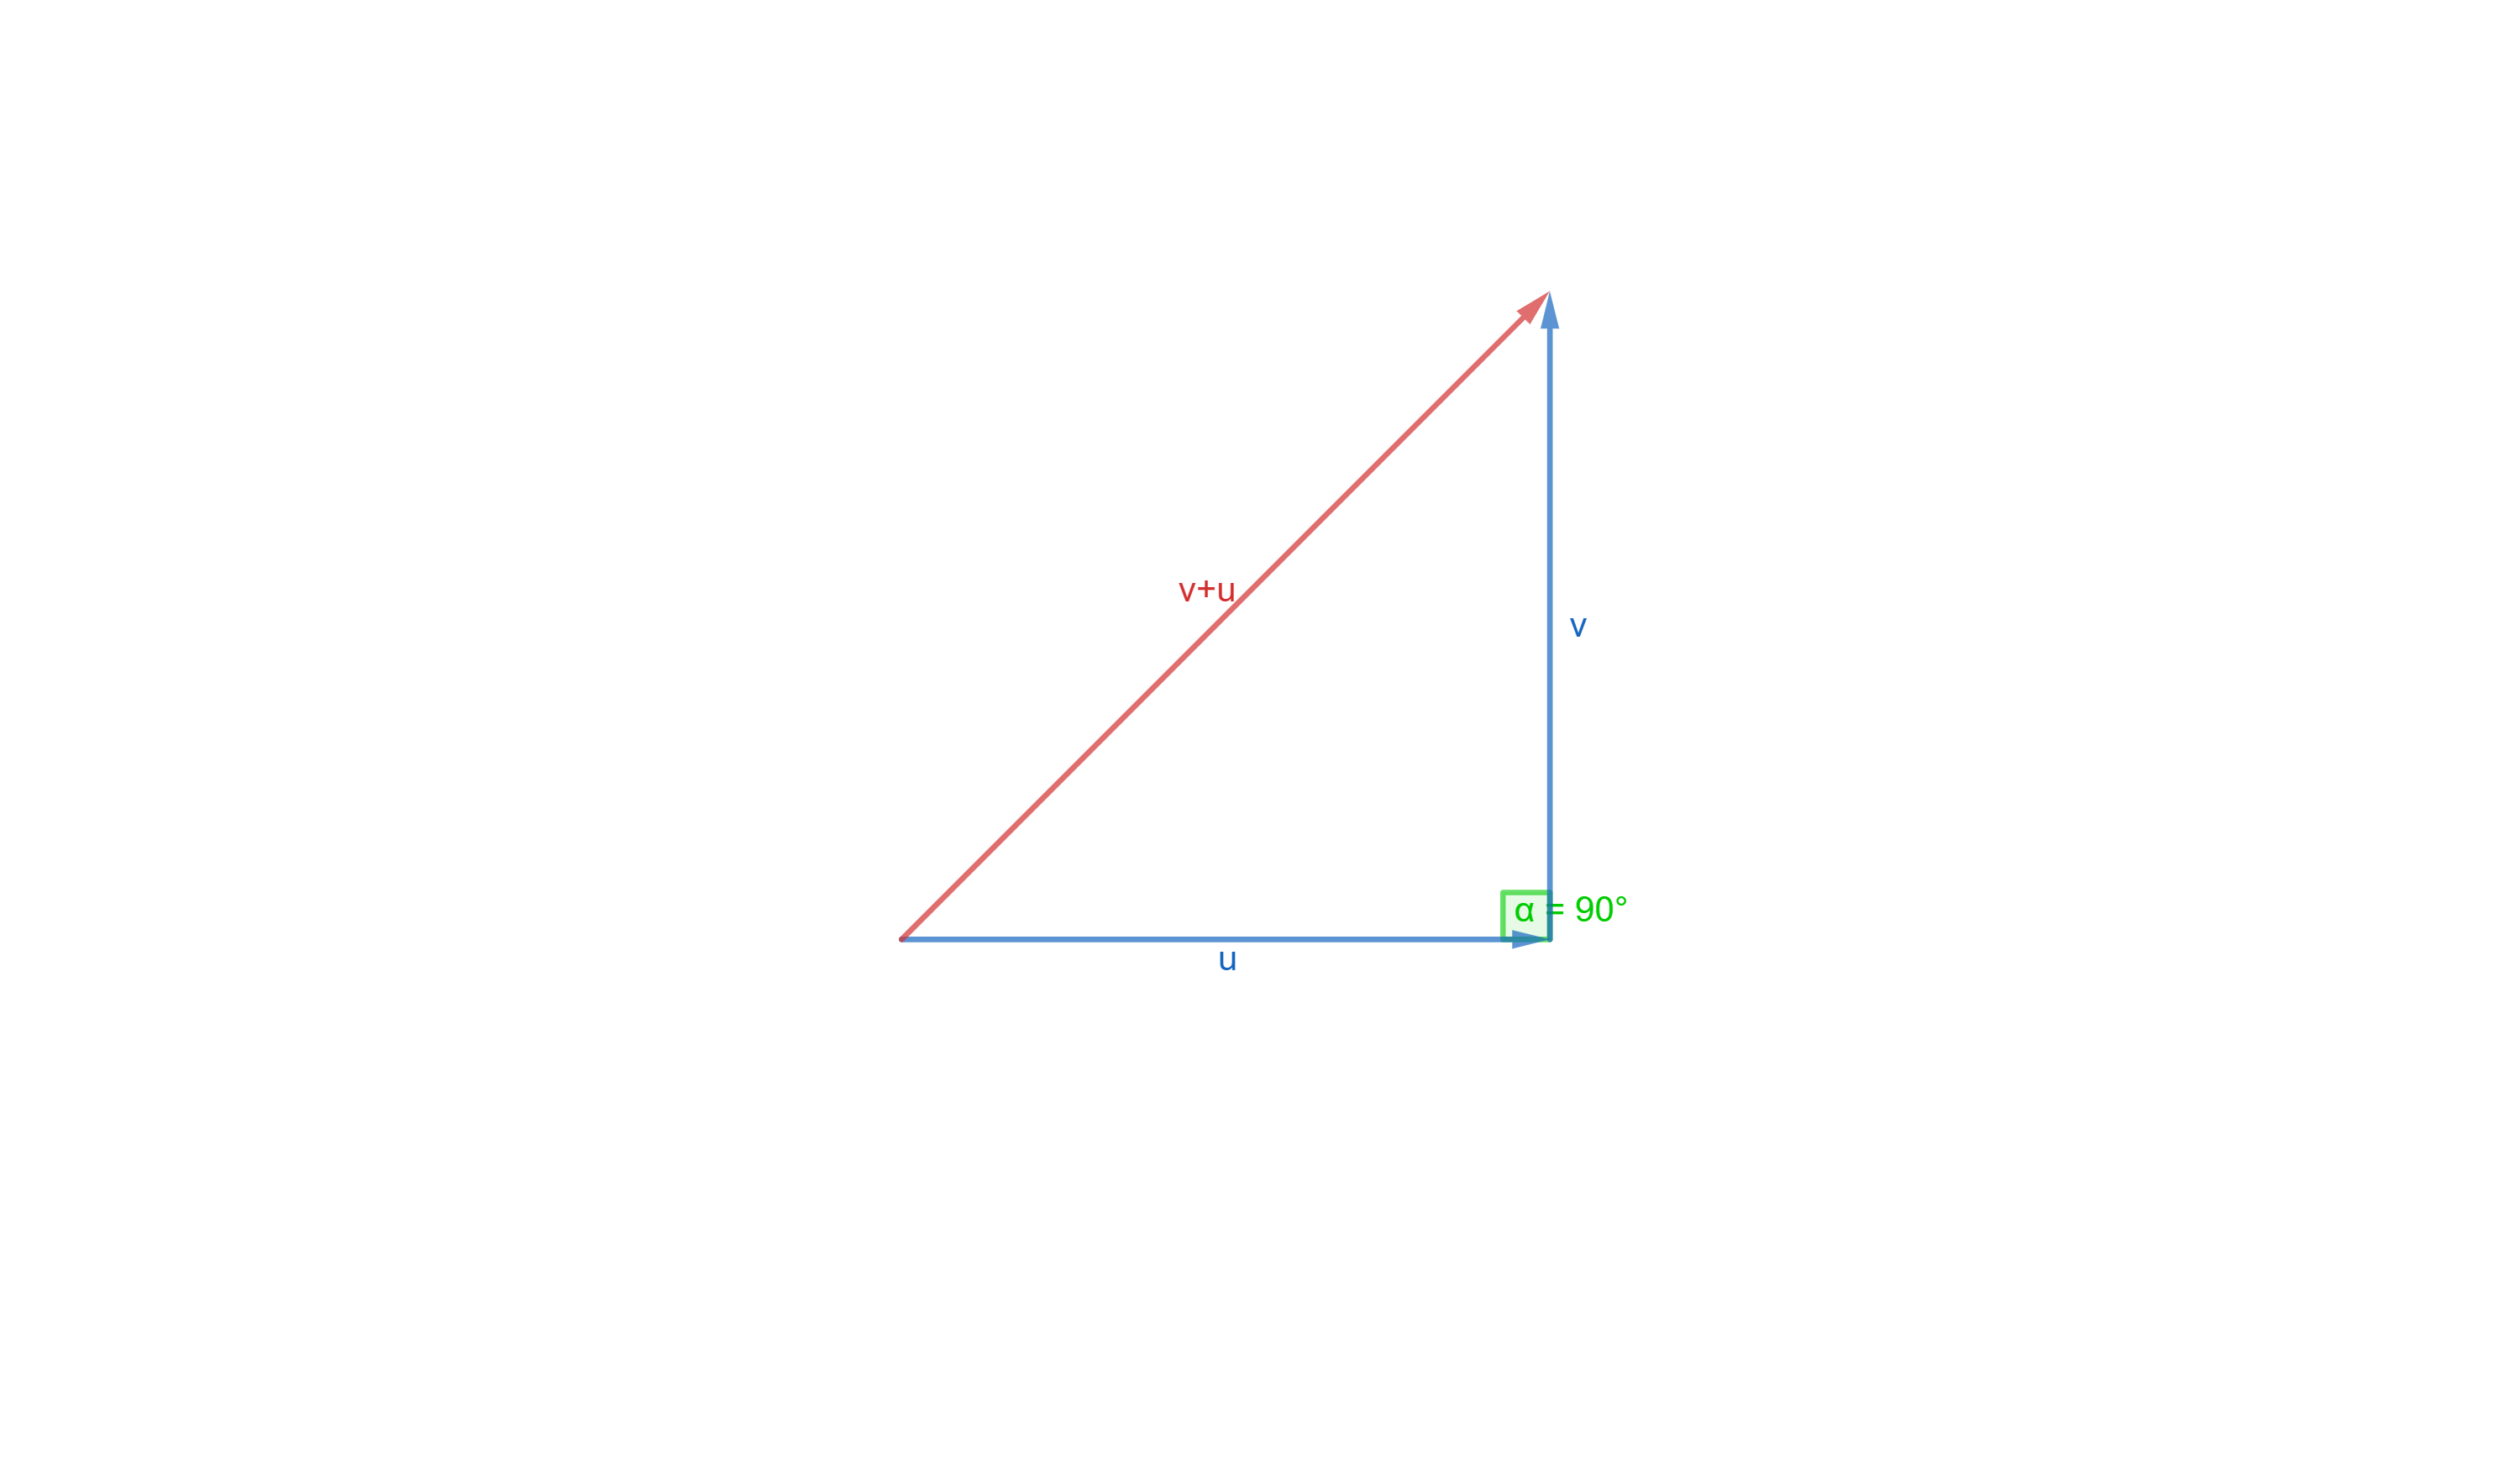
\includegraphics[width=0.7\linewidth]{imgs/alglin-06-pitagoras}
	\caption[Teorema de Pitágoras]{Teorema de Pitágoras (arquivo pessoal)}
	\label{fig:alglin-06-pitagoras}
\end{figure}

Tendo definido a ortogonalidade entre dois vetores, nós podemos começar a pensar na ortogonalidade entre dois subespaços vetoriais. A ideia é muito simples: dois subespaços serão ortogonais se todos os vetores de um subespaço forem ortogonais a todos os vetores do outro subespaço. Definindo isto formalmente:

\begin{Definition}[Subespaços vetoriais ortogonais]
	Sejam $U$ e $V$ dois subespaços vetoriais de $E$. Dizemos que $U$ é \textbf{ortogonal} a $V$ se $u\perp v$ para todos $u\in U$ e $v\in V$, e escrevemos $U\perp V$.
\end{Definition}

Uma consequência direta desta definição é o seguinte fato:

\begin{Proposition}
	Sejam $U$ e $V$ dois subespaços vetoriais de $E$ tais que $U\perp V$. Então, $w\in U\cap V$ se, e somente se, $w = 0$.
\end{Proposition}

\begin{Proof}
	$\implies$ Suponha que $w\in U\cap V$. Então, $w\in U$ e $w\in V$. Como $U\perp V$, nós temos que $w^Tw = 0$. Ou seja, $||w||^2 = 0$. No entanto, isto acontece se, e somente se, $w = 0$.
	
	$\impliedby$ Suponha que $w = 0$. Como $U$ e $V$ são subespaços vetoriais, segue que $w\in U$ e $w\in V$. Logo, $w\in U\cap V$.
	
	\qed
\end{Proof}

Vamos mostrar alguns exemplos simples que podem ser visualizados geometricamente:

\begin{Example}
	Considere $E = \mathbb{R}^2$. Então, dadas as retas $U = \{(x, x)^T; x\in\mathbb{R}\}$ e $V = \{(x, -x)^T; x\in\mathbb{R}\}$, nós temos que $U\perp V$. De fato, todo vetor de $U$ é da forma $u = \begin{bmatrix}
		a \\
		a
	\end{bmatrix}$, e todo vetor de $V$ é da forma $v = \begin{bmatrix}
		b \\
		-b
	\end{bmatrix}$. Calculando $u^Tv$, nós obtemos:
	
	$$
	u^Tv = ab + a(-b) - ab - ab = 0.
	$$
	Logo, todo vetor de $U$ é ortogonal a todo vetor de $V$. Assim sendo, segue que $U\perp V$.
\end{Example}

A figura a seguir ilustra este exemplo:

\begin{figure}[H]
	\centering
	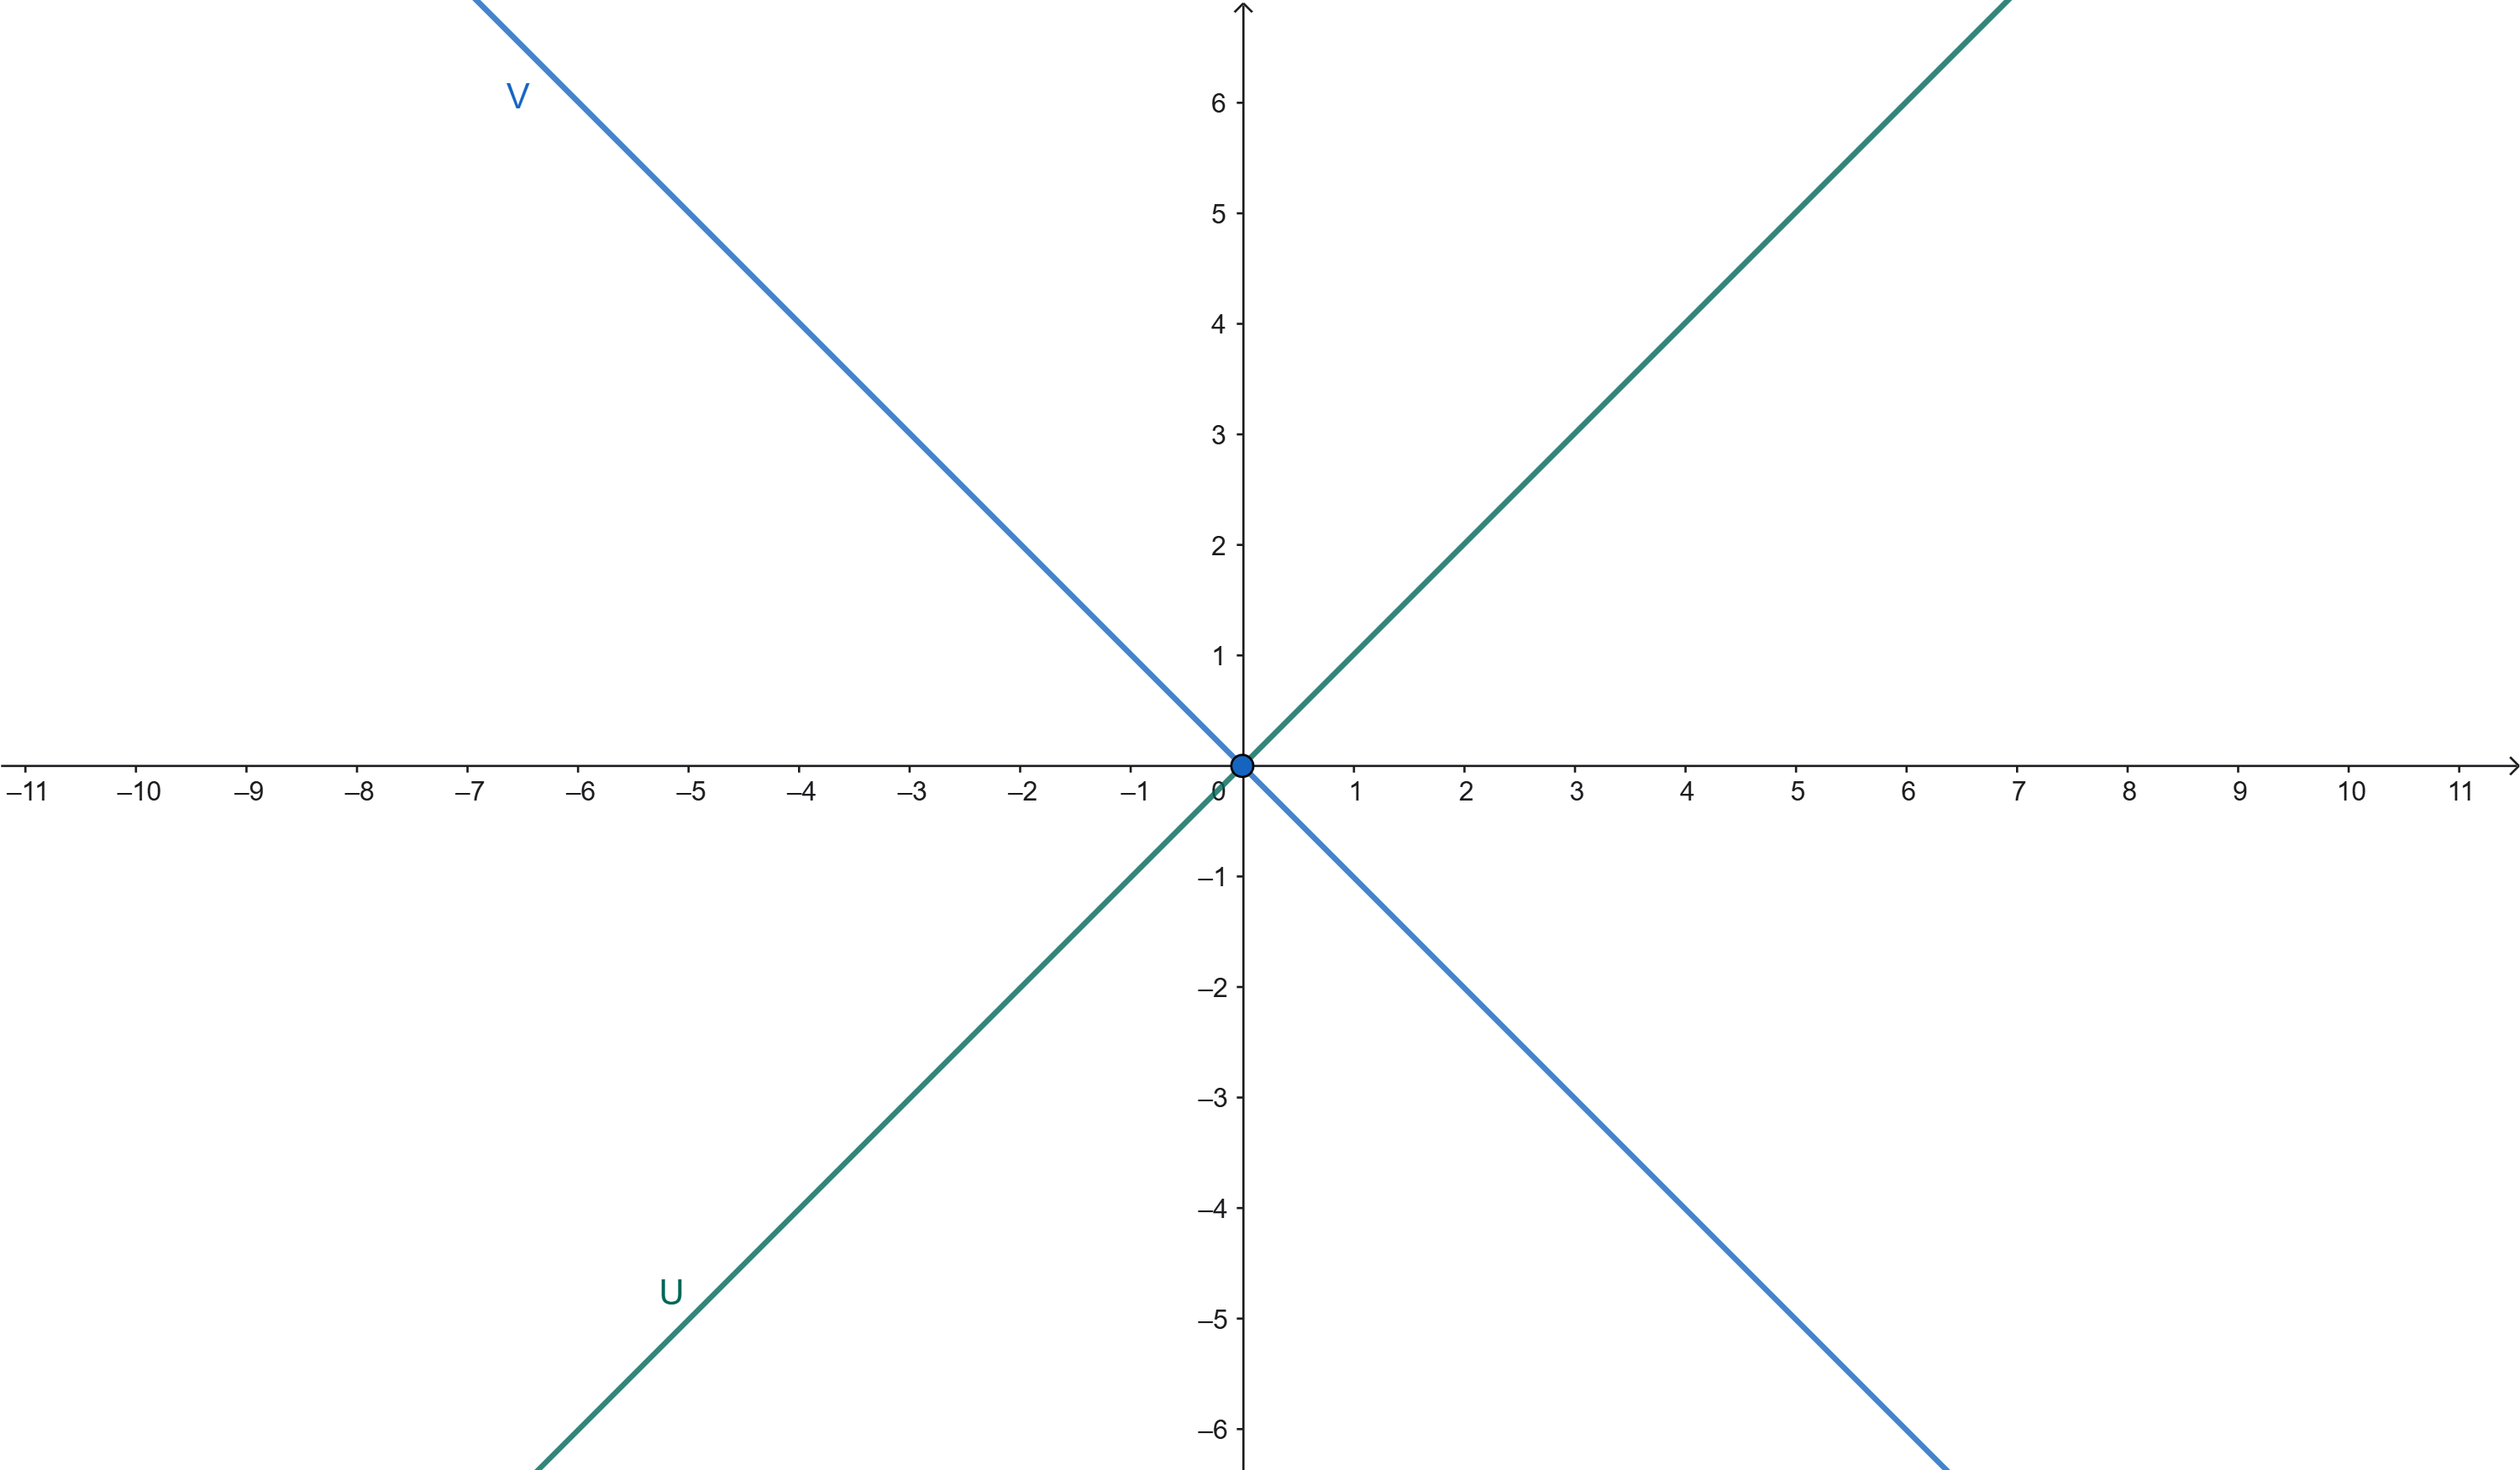
\includegraphics[width=0.7\linewidth]{imgs/alglin-07-ortogonalidade-em-r2}
	\caption[Ortogonalidade em $\mathbb{R}^2$]{Ortogonalidade em $\mathbb{R}^2$ (arquivo pessoal)}
	\label{fig:alglin-07-ortogonalidade-em-r2}
\end{figure}

\begin{Example}
	Considere $E = \mathbb{R}^3$. Então, dados o plano $U = \{(x, y, 0)^T; x,y\in\mathbb{R}\}$ e a reta $V = \{(0, 0, z)^T; z\in\mathbb{R}\}$, nós temos que $U\perp V$. De fato, todo vetor de $U$ é da forma $u = \begin{bmatrix}
		a \\
		b \\
		0
	\end{bmatrix}$ e todo vetor de $v = \begin{bmatrix}
		0 \\
		0 \\
		c
	\end{bmatrix}$. Calculando $u^Tv$, nós obtemos:
	
	$$
	u^Tv = a\cdot 0 + b\cdot 0 + 0\cdot c = 0.
	$$
	Logo, todo vetor de $U$ é ortogonal a todo vetor de $V$. Assim sendo, segue que $U\perp V$.
\end{Example}

A figura a seguir ilustra este exemplo:

\begin{figure}[H]
	\centering
	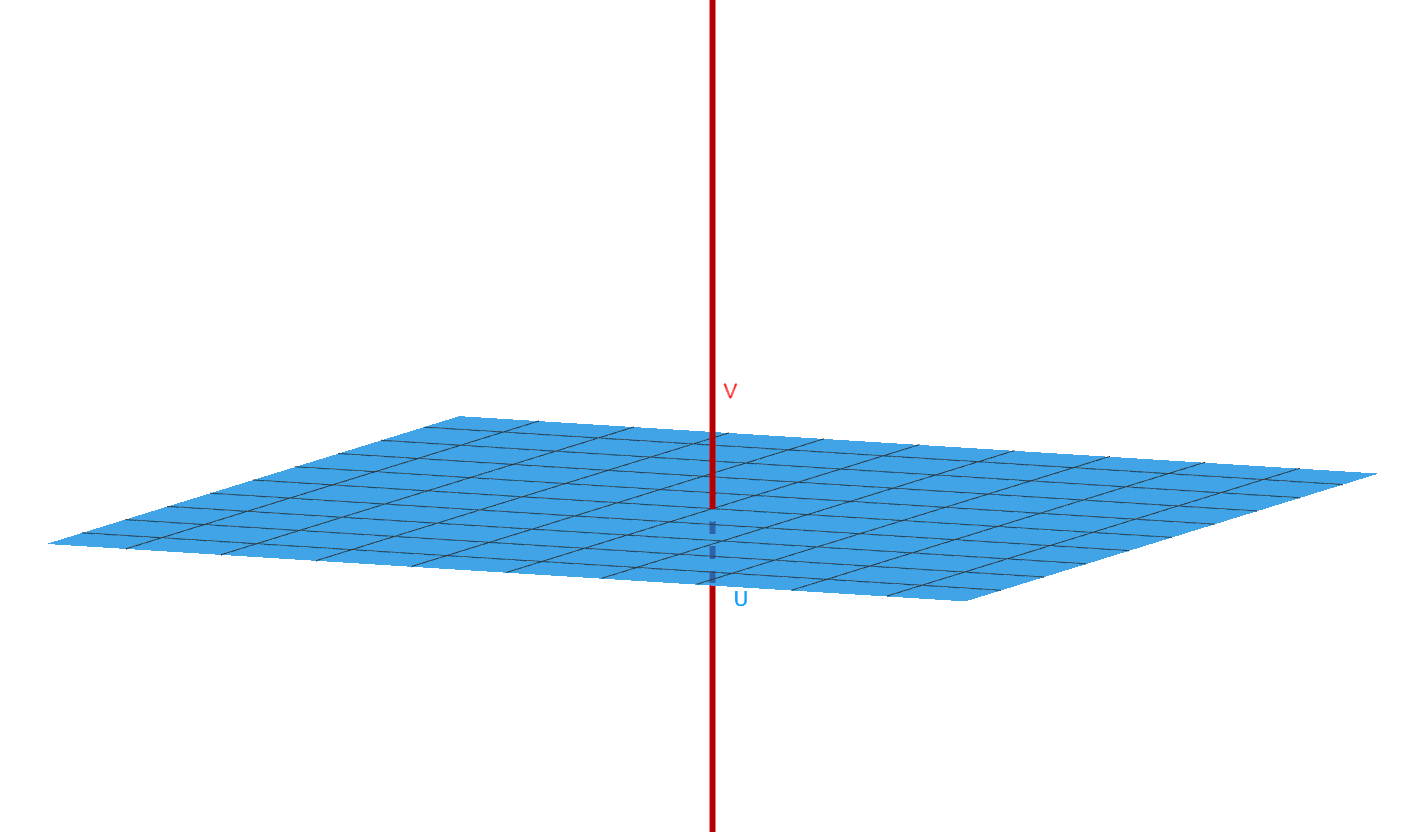
\includegraphics[width=0.7\linewidth]{imgs/alglin-08-ortogonalidade-em-r3}
	\caption[Ortogonalidade em $\mathbb{R}^3$]{Ortogonalidade em $\mathbb{R}^3$ (arquivo pessoal)}
	\label{fig:alglin-08-ortogonalidade-em-r3}
\end{figure}

Vamos agora nos voltar para os quatro subespaços fundamentais de uma matriz. No capítulo 4, nós estudamos as suas dimensões e, agora, nós estudaremos as relações de ortogonalidade entre eles. Unindo as suas relações de dimensão e de ortogonalidade, nós obtemos o que foi popularizado por Gilbert Strang como ``Teorema Fundamental da Álgebra Linear''. Como, porém, aqui eu quero tratar apenas sobre as relações de ortogonalidade, eu ainda não darei este nome e, no final do capítulo, eu enunciarei as duas partes do Teorema Fundamental da Álgebra Linear (sem fazer a sua demonstração, pois já a teremos feito em diferentes partes destas notas de aula).

\begin{Theorem}[Teorema Fundamental da Ortogonalidade]
	Seja $A$ uma matriz $m\times n$ qualquer. Então, $N(A)\perp C(A^T)$ e $C(A)\perp N(A^T)$.
\end{Theorem}

\begin{Proof}
	Primeiro, nós queremos demonstrar que $N(A)\perp C(A^T)$. Para isso, seja $w\in C(A^T)$. Então, existe $y\in\mathbb{R}^m$ tal que $w = A^Ty$. Assim sendo, tomando $x\in N(A)$ qualquer, nós temos que:
	
	$$
	x^Tw = x^TA^Ty =(Ax)^Ty = 0^Ty = 0.
	$$
	Logo, $N(A)\perp C(A^T)$.
	
	Agora, nós queremos demonstrar que $C(A)\perp N(A^T)$. Mas isto segue diretamente do primeiro fato. Nós temos que:
	
	$$
	N(A^T)\perp C((A^T)^T) = C(A).
	$$
	Logo, $N(A^T)\perp C(A)$.
	
	\qed
\end{Proof}

\section{Complemento Ortogonal}

Nesta seção, nós desenvolveremos o conceito de complemento ortogonal. O complemento ortogonal é muito simples: dado um subespaço vetorial $V$, o seu complemento ortogonal é um conjunto $W$ cujos vetores são ortogonais a $V$. Definindo de maneira mais formal:

\begin{Definition}[Complemento ortogonal]
	Seja $V$ um subespaço vetorial de $E$. Então, definimos o \textbf{complemento ortogonal} de $V$ como:
	
	$$
	V^\perp = \{w\in E; w\perp V\}.
	$$
\end{Definition}

O primeiro resultado a respeito do complemento ortogonal é bastante intuitivo: ele é também um subespaço vetorial.

\begin{Proposition}
	Seja $V$ um subespaço vetorial de $E$. Então, $V^\perp$ é também um subespaço vetorial de $E$.
\end{Proposition}

\begin{Proof}
	Considere dois vetores $w_1, w_2\in V^\perp$ e dois escalares $\alpha, \beta\in\mathbb{R}$. Nós queremos provar que $\alpha w_1 + \beta w_2\in V^\perp$. Ou seja, queremos provar que, para todo $v\in V$, $\alpha w_1 + \beta w_2\perp v$. De fato, calculando $v^T(\alpha w_1 + \beta w_2)$, nós temos que:
	
	$$
	v^T(\alpha w_1 + \beta w_2) = \alpha v^Tw_1 + \beta v^Tw_2 = \alpha\cdot 0 + \beta\cdot 0 = 0.
	$$
	Logo, nós temos que $\alpha w_1 + \beta w_2\perp v$ para todo $v\in V$, e portanto, $\alpha w_1 + \beta w_2\in V^\perp$.
	
	\qed
\end{Proof}

O fato de $V^\perp$ ser também um subespaço de $E$ nos sugere uma decomposição para qualquer vetor de $E$ que nós discutiremos no futuro. Mas vamos com calma, tudo tem o seu tempo certo. Por agora, vamos desenvolver mais alguns fatos sobre o complemento ortogonal de um subespaço, e depois estaremos prontos para falar melhor sobre isso.

\begin{Proposition}
	Seja $\{v_1, \cdots, v_k\}$ uma base para $V$. Então, $w\in V^\perp$, se, e somente se, $w\perp v_i$, para todo $i\in\{1, \cdots, k\}$.
\end{Proposition}

\begin{Proof}
	$\implies$ É verdade diretamente da definição de $V^\perp$.
	
	$\impliedby$ Suponha que $w\perp v_i$, para todo $i\in\{1, \cdots, k\}$. Queremos provar que $w\perp\operatorname{span}(\{v_1, \cdots, v_k\}) = V$. De fato, seja $v\in\operatorname{span}(\{v_1, \cdots, v_k\})$. Então, existem $c_1, \cdots, c_k\in\mathbb{R}$ tais que $v = c_1v_1 + \cdots + c_kv_k$. Calculando $w^Tv$, nós temos:
	
	$$
	w^Tv = w^T(c_1v_1 + \cdots + c_kv_k) = c_1w^Tv_1 + \cdots + c_kw^Tv_k = c_1\cdot 0 + \cdots + c_k\cdot 0 = 0. 
	$$
	Logo, pela definição, $w\in V^\perp$.
	
	\qed
\end{Proof}

Ainda considerando $\{v_1, \cdots, v_k\}$ como uma base para $V$, nós podemos, a partir deste conjunto, encontrar uma base para $V^\perp$. De fato, definamos

$$
A = \begin{bmatrix}
	- & v_1^T & - \\
	- & v_2^T & - \\
	& \vdots & \\
	- & v_k^T & -
\end{bmatrix}.
$$

Suponha que $x\in N(A)$. Então, nós temos que

$$
\begin{bmatrix}
	- & v_1^T & - \\
	- & v_2^T & - \\
	& \vdots & \\
	- & v_k^T & -
\end{bmatrix}x = 0,
$$
o que nos dá $v_i^Tx = 0$ para cada $v_i$. Logo, se $x\in N(A)$, então $x\in V^\perp$ e, reciprocamente, se $x\in V^\perp$, então $v_i^Tx = 0$ para cada $v_i$, e, portanto, $x\in N(A)$. Assim sendo, nós temos que $V^\perp = N(A)$ e, portanto, para encontrarmos uma base para $V^\perp$, basta encontrar uma base para $N(A)$. Nós já sabemos fazer isso: basta encontrar a matriz núcleo $N$.

\begin{Example}
	Seja $V = \operatorname{span}\left(\left\{\begin{bmatrix}
		1 \\
		0 \\
		1 \\
		0
	\end{bmatrix}, \begin{bmatrix}
		1 \\
		2 \\
		3 \\
		4
	\end{bmatrix}\right\}\right)$ um subespaço de $\mathbb{R}^4$. Como o conjunto $\left\{\begin{bmatrix}
		1 \\
		0 \\
		1 \\
		2
	\end{bmatrix}, \begin{bmatrix}
		1 \\
		2 \\
		3 \\
		4
	\end{bmatrix}\right\}$ é LI, nós temos que ele é uma base para $V$. Nós queremos encontrar uma base para $V^\perp$. Para fazer isto, definamos a matriz $A$ como:
	
	$$
	A = \begin{bmatrix}
		1 & 0 & 1 & 2 \\
		1 & 2 & 3 & 4
	\end{bmatrix}.
	$$
	Fazendo o processo de escalonamento, nós obtemos:
	
	$$
	\begin{bmatrix}
		1 & 0 & 1 & 2 \\
		1 & 2 & 3 & 4
	\end{bmatrix}\overset{L_2 - L_1}{\implies}\begin{bmatrix}
		1 & 0 & 1 & 2 \\
		0 & 2 & 2 & 2
	\end{bmatrix}\overset{L_2/2}{\implies}\begin{bmatrix}
		1 & 0 & 1 & 2 \\
		0 & 1 & 1 & 1
	\end{bmatrix} = R.
	$$
	Nós temos que $F = \begin{bmatrix}
		1 & 2 \\
		1 & 1
	\end{bmatrix}$, e, como nós não fizemos nenhuma permutação entre colunas, $R = R'$ e $N = N'$. Assim sendo, a matriz núcleo é dada por:
	
	$$
	N = \begin{bmatrix}
		-1 & -2 \\
		-1 & -1 \\
		1 & 0 \\
		0 & 1
	\end{bmatrix}.
	$$
	Logo, o conjunto $\left\{\begin{bmatrix}
		-1 \\
		-1 \\
		1 \\
		0
	\end{bmatrix}, \begin{bmatrix}
		-2 \\
		-1 \\
		0 \\
		1
	\end{bmatrix}\right\}$ é uma base para $V^\perp$.
\end{Example}

Agora, nós vamos enunciar e demonstrar mais três proposições antes de chegarmos à tão sonhada decomposição ortogonal (este é nome da decomposição de que falamos anteriormente).

\begin{Proposition}
	Seja $V$ um subespaço vetorial de $E$. Então, $V\cap V^\perp = \{0\}$.
\end{Proposition}

\begin{Proof}
	$\implies$ Considere um vetor $w$ tal que $w\in V\cap V^\perp$. Então, $w\in V$ e $w\in V^\perp$. Assim sendo, $w\perp w$, ou seja, $w^Tw = 0$. Segue que $||w||^2 = 0$, o que acontece se, e somente se, $w = 0$.
	
	$\impliedby$ Nós sabemos que, dado um subespaço qualquer $U$, $0\in U$. Assim sendo, como $V\cap V^\perp$ é um subespaço vetorial (em algum exercício anterior pede-se para provar este fato), nós temos que $0\in V\cap V^\perp$. Logo, $\{0\}\subseteq V\cap V^\perp$.
	
	Logo, $V\cap V^\perp = \{0\}$.
	
	\qed
\end{Proof}

\begin{Proposition}
	Seja $V$ um subespaço vetorial de $E$. Então, $\dim V + \dim V^\perp = \dim E$.
\end{Proposition}

\begin{Proof}
	Suponha que $\{v_1, \cdots, v_r\}$ é uma base para $V$, com $\dim V = r$ e $\dim E = n$. Então, como nós vimos anteriormente, nós temos que $V^\perp = N(A)$, onde
	
	$$
	A = \begin{bmatrix}
		- & v_1^T & - \\
		- & v_2^T & - \\
		& \vdots & \\
		- & v_r^T & - \\
	\end{bmatrix}.
	$$
	Assim sendo, nós temos que $\dim C(A^T) = r$ e, consequentemente, $\dim C(A) = r$ também. Logo, segue que $\dim N(A) = n - r$. Mas como $V^\perp = N(A)$, nós temos que $\dim V + \dim V^\perp = r + (n - r) = n = \dim E$.
	
	\qed
\end{Proof}

\begin{Proposition}
	Seja $V$ um espaço vetorial de $E$. Então, $V = (V^\perp)^\perp$.
\end{Proposition}

\begin{Proof}
	Primeiramente, nós vamos demonstrar que $V\subseteq(V^\perp)^\perp$. Para isso, tome $u\in V$. Por definição, para qualquer $v\in V^\perp$, nós temos que $u^Tv = 0$. Nós sabemos que o produto interno é simétrico por definição, logo, $u^Tv = v^Tu$. Como $u^Tv = 0$, segue que $v^Tu = 0$. Logo, nós temos que $u\perp V^\perp$. Portanto, $u\in(V^\perp)^\perp$. Assim sendo, $V\subseteq(V^\perp)^\perp$.
	
	Agora, nós queremos demonstrar que $(V^\perp)^\perp = V$. Para fazer isso, vamos usar as dimensões dos subespaços. Por um lado, nós temos que $\dim V + \dim V^\perp = \dim E$. Por outro lado, nós temos que $\dim V^\perp + \dim (V^\perp)^\perp = \dim E$. Assim sendo, nós temos que:
	
	$$
	\dim V + \dim V^\perp = \dim V^\perp + \dim (V^\perp)^\perp \implies \dim V = \dim (V^\perp)^\perp.
	$$
	Como $V$ é um subespaço de $(V^\perp)^\perp$ (como nós demonstramos acima), e $V$ possui a mesma dimensão de $(V^\perp)^\perp$, segue que $V = (V^\perp)^\perp$.
	
	\qed
\end{Proof}

Estamos prontos para falar em decomposição ortogonal. Em exercícios anteriores, nós definimos e trabalhamos com a soma de dois subespaços. No entanto, a fim de formalizar melhor esta ideia, nós iremos definir este conceito novamente.

\begin{Definition}[Soma de dois subespaços]
	Sejam $V_1$ e $V_2$ dois subespaços vetoriais de $V$. Então, nós definimos a \textbf{soma} de $V_1$ e $V_2$ como:
	
	$$
	V_1 + V_2 = \{v_1 + v_2; v_1\in V_1 \text{ e } v_2\in V_2\}.
	$$
\end{Definition}

Como esta ideia nos sugere, este conceito pode ser estendido para a soma de $m$ subespaços de $V$, da seguinte forma:

\begin{Definition}[Soma de $m$ subespaços]
	Sejam $V_1, \cdots, V_m$ subespaços vetoriais de $V$. Então, nós definimos a \textbf{soma} de $V_1, \cdots, V_m$ como:
	
	$$
	V_1 + \cdots + V_m = \{v_1 + \cdots + v_m; v_1\in V_1, \cdots, v_m\in V_m\}.
	$$
\end{Definition}

No nosso caso, nós estamos preocupados especificamente com o caso $m = 2$. Mas antes de chegar ao que queremos, nós definiremos, ainda para uma quantidade qualquer de subespaços, a soma direta.

\begin{Definition}[Soma direta]
	Sejam $V_1, \cdots, V_m$ subespaços de $V$ tais que cada vetor de $V_1 + \cdots + V_m$ pode ser escrito de forma única como $v_1 + \cdots + v_m$. Então, dizemos que esta soma é uma \textbf{soma direta}, e a denotamos por $V_1\oplus\cdots\oplus V_m$.
\end{Definition}

Com estas coisas em mente, vamos agora enunciar e demonstrar o Teorema da Decomposição Ortogonal.

\begin{Theorem}[Teorema da Decomposição Ortogonal]
	Seja $V$ um subespaço vetorial de $E$. Então, todo vetor $x\in E$ pode ser escrito, de forma única, como $x = v + v^\perp$, onde $v\in V$ e $v^\perp\in V^\perp$.
\end{Theorem}

\begin{Proof}
	\textbf{Existência:} Suponha que $\dim E = n$ e $\dim V = k$. Então, consideremos as bases $\{v_1, \cdots, v_k\}$ e $\{w_1, \cdots, w_{n - k}\}$ para $V$ e $V^\perp$, respectivamente. Nós provaremos que o conjunto $\{v_1, \cdots, v_k, w_1, \cdots, w_{n - k}\}$ é LI. De fato, tomemos
	
	$$
	\alpha_1v_1 + \cdots + \alpha_kv_k + \alpha_{k + 1}w_1 + \cdots + \alpha_nw_{n-k} = 0.
	$$ 
	Nós temos que
	
	$$
	\alpha_1v_1 + \cdots + \alpha_kv_k = -(\alpha_{k + 1}w_1 + \cdots + \alpha_nw_{n - k}).
	$$ 
	O lado esquerdo da equação pertence a $V$, e o lado direito da equação pertence a $V^\perp$. Logo, ambos os vetores pertencem a $V\cap V^\perp$. Mas nós sabemos que $V\cap V^\perp = \{0\}$. Logo:
	
	$$
	\alpha_1v_1 + \cdots + \alpha_kv_k = 0
	$$
	e
	
	$$
	\alpha_{k + 1}w_1 + \cdots + \alpha_nw_{n - k} = 0.
	$$
	Pela independência linear dos $v_i$'s e dos $w_i$'s, segue que:
	
	$$
	\alpha_1 = \cdots = \alpha_k = \alpha_{k + 1} = \cdots = \alpha_n = 0.
	$$
	
	Logo, o conjunto $\{v_1, \cdots, v_k, w_1, \cdots, w_{n - k}\}$ é LI. Mais do que isso, como este conjunto possui $n$ vetores e $\dim E = n$, ele é uma base para $E$. Assim sendo, para todo $x\in E$, existem $\alpha_1, \cdots, \alpha_k, \alpha_{k + 1}, \cdots, \alpha_n\in\mathbb{R}$ tais que:
	
	$$
	x = \alpha_1v_1 + \cdots + \alpha_kv_k + \alpha_{k + 1}w_1 + \cdots + \alpha_nw_{n - k}.
	$$
	Ou seja, $x = v + v^\perp$.
	
	\textbf{Unicidade:} Suponha que existem $v_1, v_2\in V$ e $v_1^\perp, v_2^\perp\in V^\perp$ tais que
	
	$$
	x = v_1 + v_1^\perp = v_2 + v_2^\perp.
	$$
	Então, segue que $v_1 - v_2 = v_2^\perp - v_1^\perp$. O primeiro vetor pertence a $V$ e o segundo vetor pertence a $V^\perp$. Logo, ambos os vetores pertencem a $V\cap V^\perp = \{0\}$. Ou seja, $v_1 - v_2 = 0$ e $v_2^\perp - v_1^\perp = 0$. Segue então que $v_1 = v_2$ e $v_1^\perp = v_2^\perp$.
	
	\qed
\end{Proof}

Do Teorema da Decomposição Ortogonal, segue imediatamente o seguinte corolário:

\begin{Corolary}
	Seja $V$ um subespaço vetorial de $E$. Então, $E = V\oplus V^\perp$.
\end{Corolary}

A grande importância que tem o Teorema da Decomposição Ortogonal é a ideia de projeção ortogonal, que desenvolveremos a partir da próxima seção. Mas, antes disso, façamos um exemplo para mostrar como podemos encontrar a decomposição ortogonal de um vetor dados um subespaço e o seu complemento ortogonal.

\begin{Example}
	Considere $x = \begin{bmatrix}
		2 \\
		5 \\
		-1 \\
		0
	\end{bmatrix}$ e o subespaço vetorial $V = \operatorname{span}\left(\left\{\begin{bmatrix}
		1 \\
		0 \\
		1 \\
		0
	\end{bmatrix}, \begin{bmatrix}
		0 \\
		1 \\
		2 \\
		4
	\end{bmatrix}\right\}\right)$. Nós queremos encontrar os vetores $v\in V$ e $v^\perp\in V^\perp$ tais que $x = v + v^\perp$. Primeiramente, vamos encontrar uma base para $V^\perp$, sabendo que o conjunto $\left\{\begin{bmatrix}
		1 \\
		0 \\
		1 \\
		0
	\end{bmatrix}, \begin{bmatrix}
		0 \\
		1 \\
		2 \\
		4
	\end{bmatrix}\right\}$ é uma base para $V$. Montando a matriz $A$, nós temos:
	
	$$
	A = \begin{bmatrix}
		1 & 0 & 1 & 0 \\
		0 & 1 & 2 & 4
	\end{bmatrix}.
	$$
	A matriz $A$ já está na sua forma escalonada reduzida. Assim sendo, nós temos que:
	
	$$
	N = \begin{bmatrix}
		-1 & 0 \\
		-2 & -4 \\
		1 & 0 \\
		0 & 1
	\end{bmatrix}.
	$$
	Ou seja, $\left\{\begin{bmatrix}
		-1 \\
		-2 \\
		1 \\
		0
	\end{bmatrix}, \begin{bmatrix}
		0 \\
		-4 \\
		0 \\
		1
	\end{bmatrix}\right\}$ é uma base para $V^\perp$. Então, nós queremos encontrar escalares $a, b, c, d\in\mathbb{R}$ tais que:
	
	$$
	\begin{bmatrix}
		2 \\
		5 \\
		-1 \\
		0
	\end{bmatrix} = 
	a\begin{bmatrix}
		1 \\
		0 \\
		1 \\
		0
	\end{bmatrix} + b\begin{bmatrix}
		0 \\
		1 \\
		2 \\
		4
	\end{bmatrix} + c\begin{bmatrix}
		-1 \\
		-2 \\
		1 \\
		0
	\end{bmatrix} + d\begin{bmatrix}
		0 \\
		-4 \\
		0 \\
		1
	\end{bmatrix}
	$$
	Isto equivale ao seguinte sistema linear:
	
	$$
	\begin{bmatrix}
		1 & 0 & -1 & 0 \\
		0 & 1 & -2 & -4 \\
		1 & 2 & 1 & 0 \\
		0 & 4 & 0 & 1
	\end{bmatrix}
	\begin{bmatrix}
		a \\
		b \\
		c \\
		d
	\end{bmatrix}
	=
	\begin{bmatrix}
		2 \\
		5 \\
		-1 \\
		0
	\end{bmatrix}
	$$
	Resolvendo este sistema linear (nós não o faremos aqui, porque, a esta altura, certamente vocês já estão cansados de fazer isso, e eu também), nós obtemos:
	
	$$
	\begin{bmatrix}
		a \\
		b \\
		c \\
		d
	\end{bmatrix} = \begin{bmatrix}
		15/38 \\
		4/38 \\
		-61/38 \\
		-16/38
	\end{bmatrix}.
	$$
	Assim sendo, o vetor $v$ é dado por:
	
	$$
	v = a\begin{bmatrix}
		1 \\
		0 \\
		1 \\
		0
	\end{bmatrix} + b\begin{bmatrix}
		0 \\
		1 \\
		2 \\
		4
	\end{bmatrix} = \dfrac{15}{38}\begin{bmatrix}
		1 \\
		0 \\
		1 \\
		0
	\end{bmatrix} + \dfrac{4}{38}\begin{bmatrix}
		0 \\
		1 \\
		2 \\
		4
	\end{bmatrix} = \begin{bmatrix}
		15/38 \\
		4/38 \\
		23/38 \\
		16/38
	\end{bmatrix},
	$$
	e o vetor $v^\perp$ é dado por:
	
	$$
	v^\perp = c\begin{bmatrix}
		-1 \\
		-2 \\
		1 \\
		0
	\end{bmatrix} + d\begin{bmatrix}
		0 \\
		-4 \\
		0 \\
		1
	\end{bmatrix} = -\dfrac{61}{38}\begin{bmatrix}
		-1 \\
		-2 \\
		1 \\
		0
	\end{bmatrix} + -\dfrac{16}{38}\begin{bmatrix}
		0 \\
		-4 \\
		0 \\
		1
	\end{bmatrix} = \begin{bmatrix}
		61/38 \\
		186/38 \\
		-61/38 \\
		-16/38
	\end{bmatrix}.
	$$
	Logo, a decomposição ortogonal de $x$ é:
	
	$$
	\begin{bmatrix}
		2 \\
		5 \\
		-1 \\
		0
	\end{bmatrix} = \begin{bmatrix}
		15/38 \\
		4/38 \\
		23/38 \\
		16/38
	\end{bmatrix} + \begin{bmatrix}
		61/38 \\
		186/38 \\
		-61/38 \\
		-16/38
	\end{bmatrix},
	$$
	ou, escrevendo de um jeito mais bonitinho,
	
	$$
	\begin{bmatrix}
		2 \\
		5 \\
		-1 \\
		0
	\end{bmatrix} = \dfrac{1}{38}\left(\begin{bmatrix}
		15 \\
		4 \\
		23 \\
		16
	\end{bmatrix} + \begin{bmatrix}
		61 \\
		186 \\
		-61 \\
		-16
	\end{bmatrix}\right).
	$$
\end{Example}

\section{Matrizes de Projeção}

Nesta seção, nós vamos falar sobre matrizes de projeção. Mais especificamente, nós estaremos em falar sobre projeção ortogonal. E a primeira pergunta natural é: ``por que nós queremos projetar?'' A resposta é muito simples: nem todo sistema linear $Ax = b$ possui solução. No entanto, o nosso grande objetivo é resolver $Ax = b$. Então, quando o sistema não tem solução, nós queremos encontrar algo que se pareça com uma solução. A projeção nos dá exatamente isso.

Mas, para falar em projeção, nós precisamos primeiro entender o que é isso. Vamos começar com um caso mais simples, e depois estendemos a ideia para casos mais gerais.

Considere $a$ e $b$ dois vetores em $\mathbb{R}^2$. Para a nossa discussão ficar interessante, considere que $a$ e $b$ são vetores LI. Vamos mostrar uma figura para esta ideia ficar mais clara:

\begin{figure}[H]
	\centering
	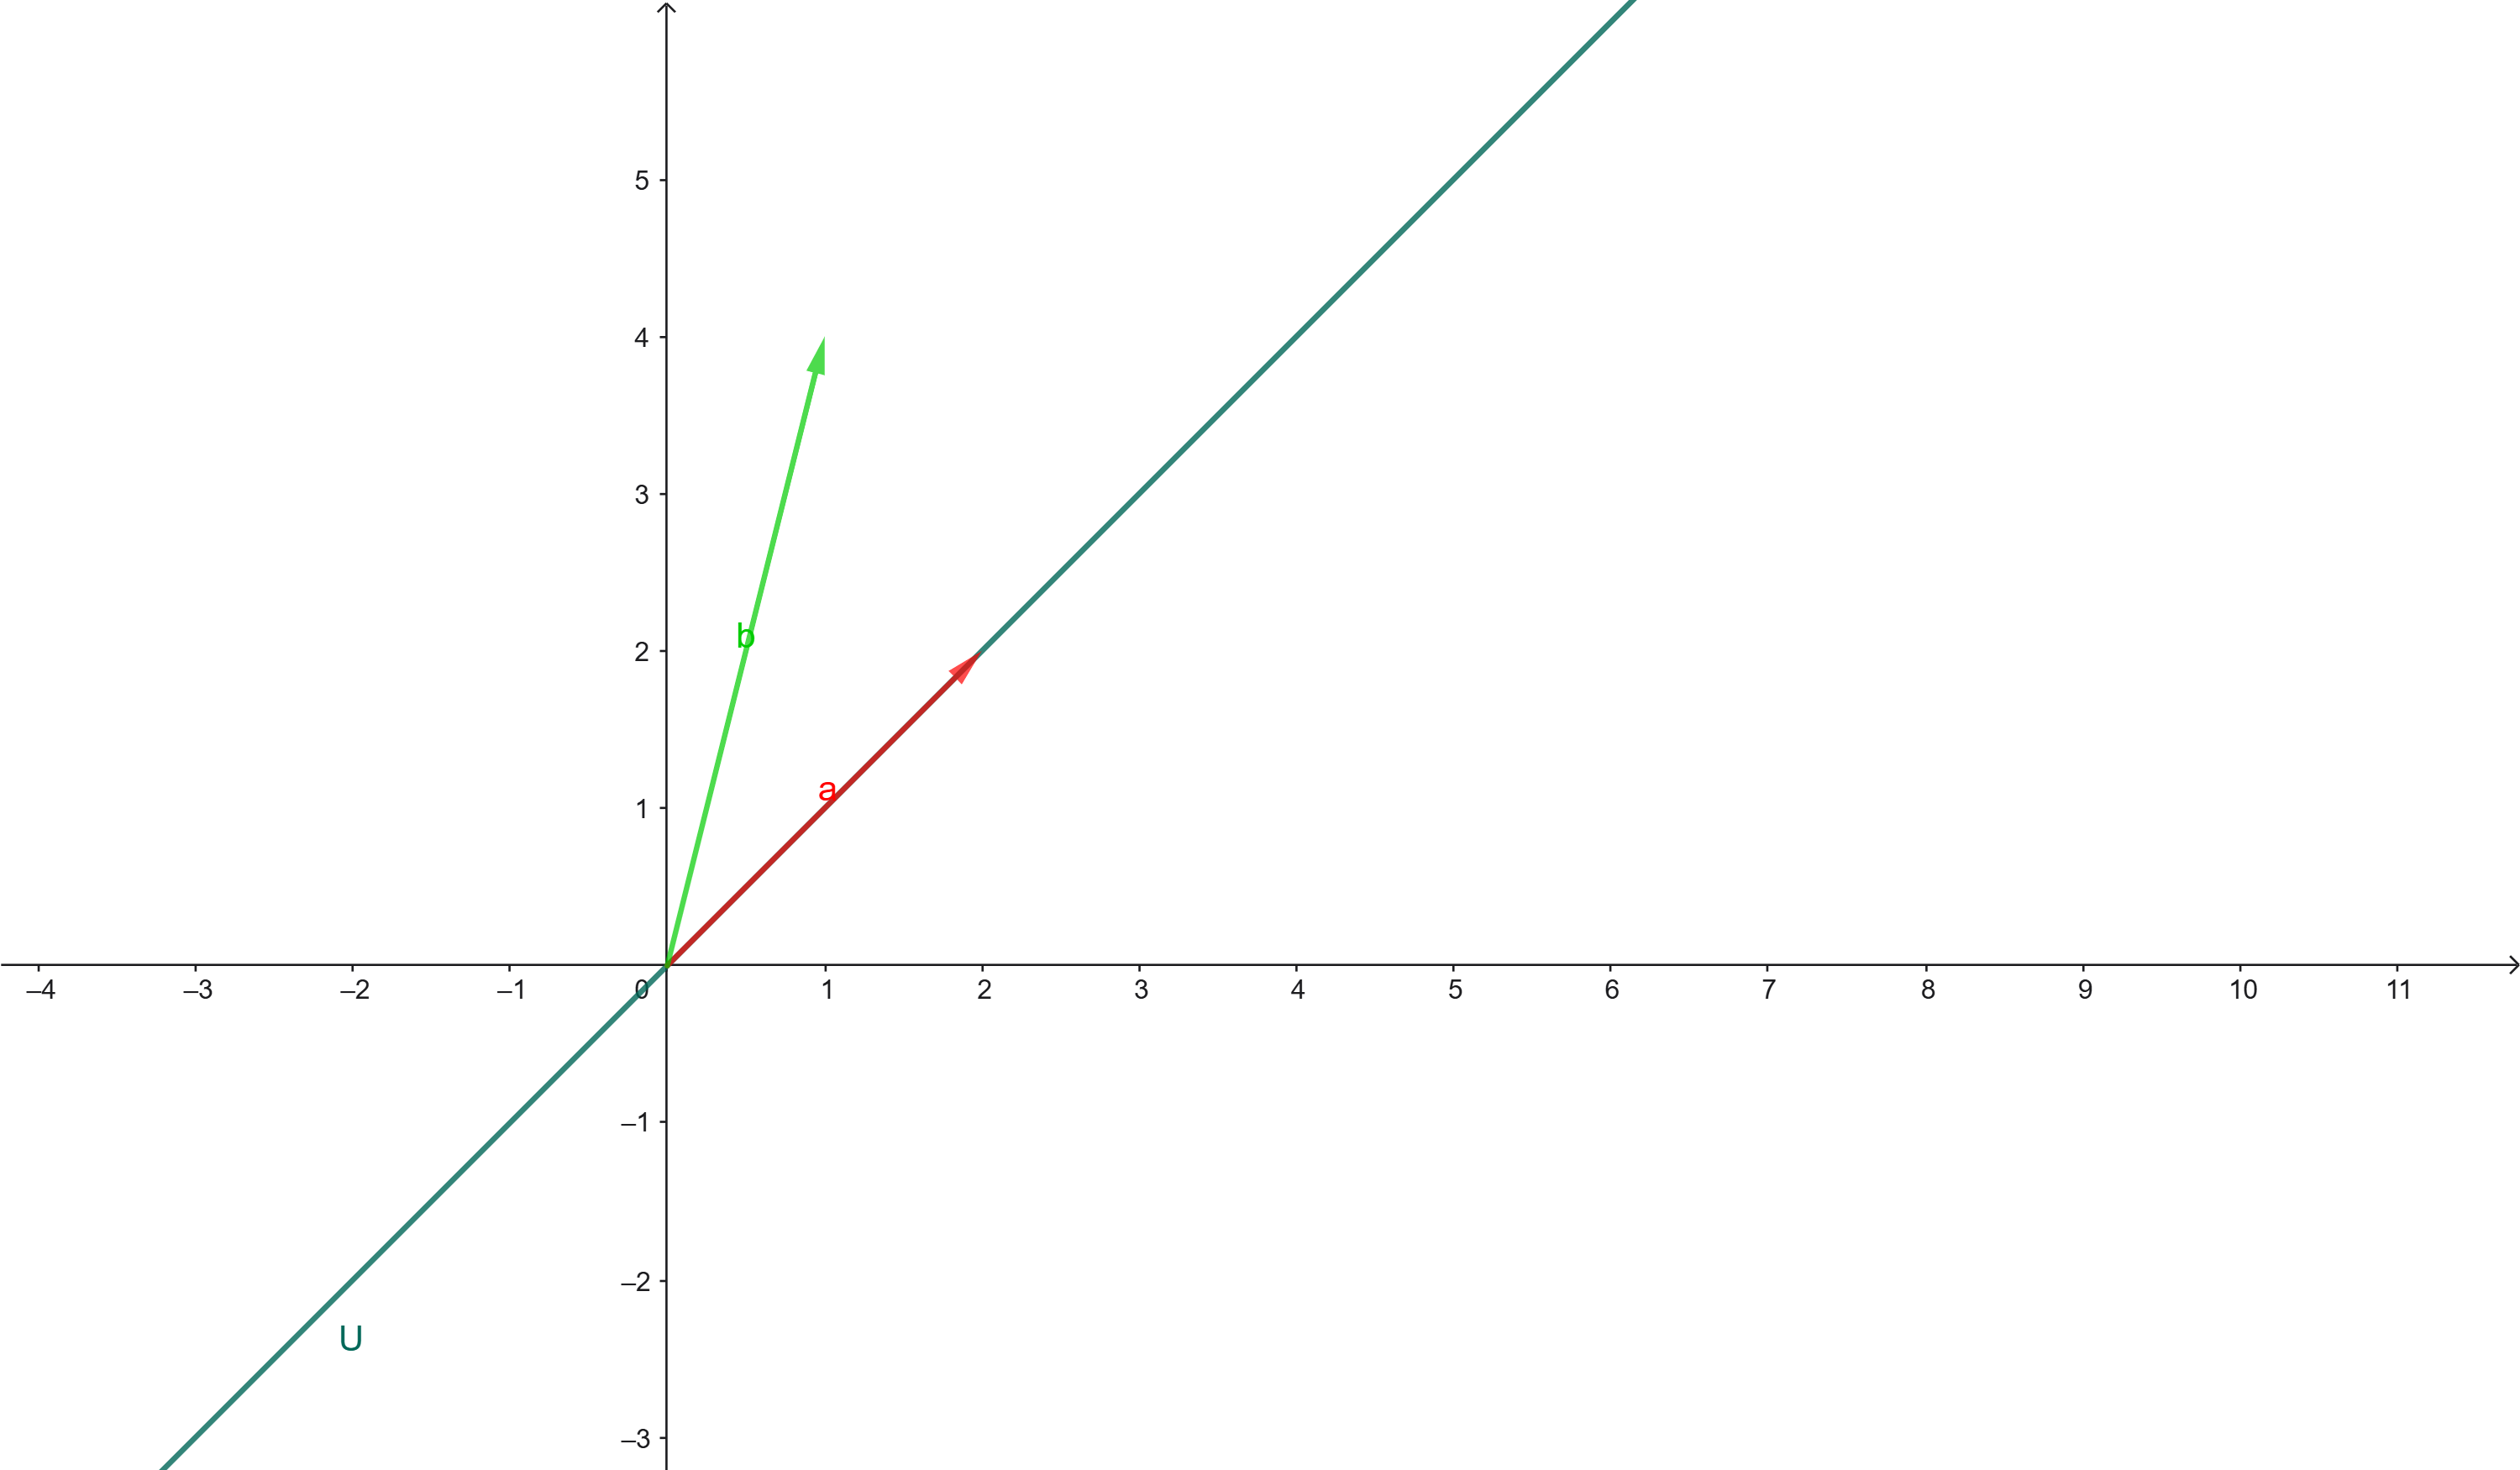
\includegraphics[width=0.7\linewidth]{imgs/alglin-09-projecao-1}
	\caption[Vetores LI em $\mathbb{R}^2$]{Vetores LI em $\mathbb{R}^2$ (arquivo pessoal)}
	\label{fig:alglin-09-projecao-1}
\end{figure}

O vetor $a$ está em um subespaço vetorial $U$, enquanto o vetor $b$ não está neste subespaço. Nós desejamos projetar $b$ em $a$, ou seja, nós queremos encontrar um vetor $p\in U$ tal que $p = xa$, para algum $x\in\mathbb{R}$, de modo que $b$ pode ser escrito como $b = p + q$, para algum $q$ em outro subespaço. Existem muitas formas de fazer isso. Na verdade, existem infinitas formas. A própria escolha $p = a$ é uma opção (dado que $b = a + (b - a)$). Então, na prática, nós já achamos uma projeção de $b$ em $a$ (ou melhor dizendo, de $b$ no subespaço $U$).

No entanto, dadas infinitas possíveis projeções, nós queremos encontrar uma projeção que seja melhor do que todas as outras. E ser melhor, no nosso caso, significa minimizar a distância entre $b$ e $p$. Ou seja, nós queremos encontrar um vetor $p$ tal que $||b - p||$ seja a menor possível. Intuitivamente (e, de maneira nada rigorosa), nós queremos um vetor $p$ que seja quase igual a $b$, só que pertencente ao subespaço $U$.

E isto é algo bastante sugestivo: nós sabemos que, em $\mathbb{R}^2$ (e, na prática, em $\mathbb{R}^n$), a melhor forma de fazer isso é encontrar um vetor $p$ tal que $b - p$ seja ortogonal a $a$ (e a $p$ também, mas enfim). Ou seja, nós queremos encontrar um vetor $p$ tal que $a^T(b - p) = 0$. Novamente, vamos ver uma imagem para estas ideias ficarem mais claras:

\begin{figure}[H]
	\centering
	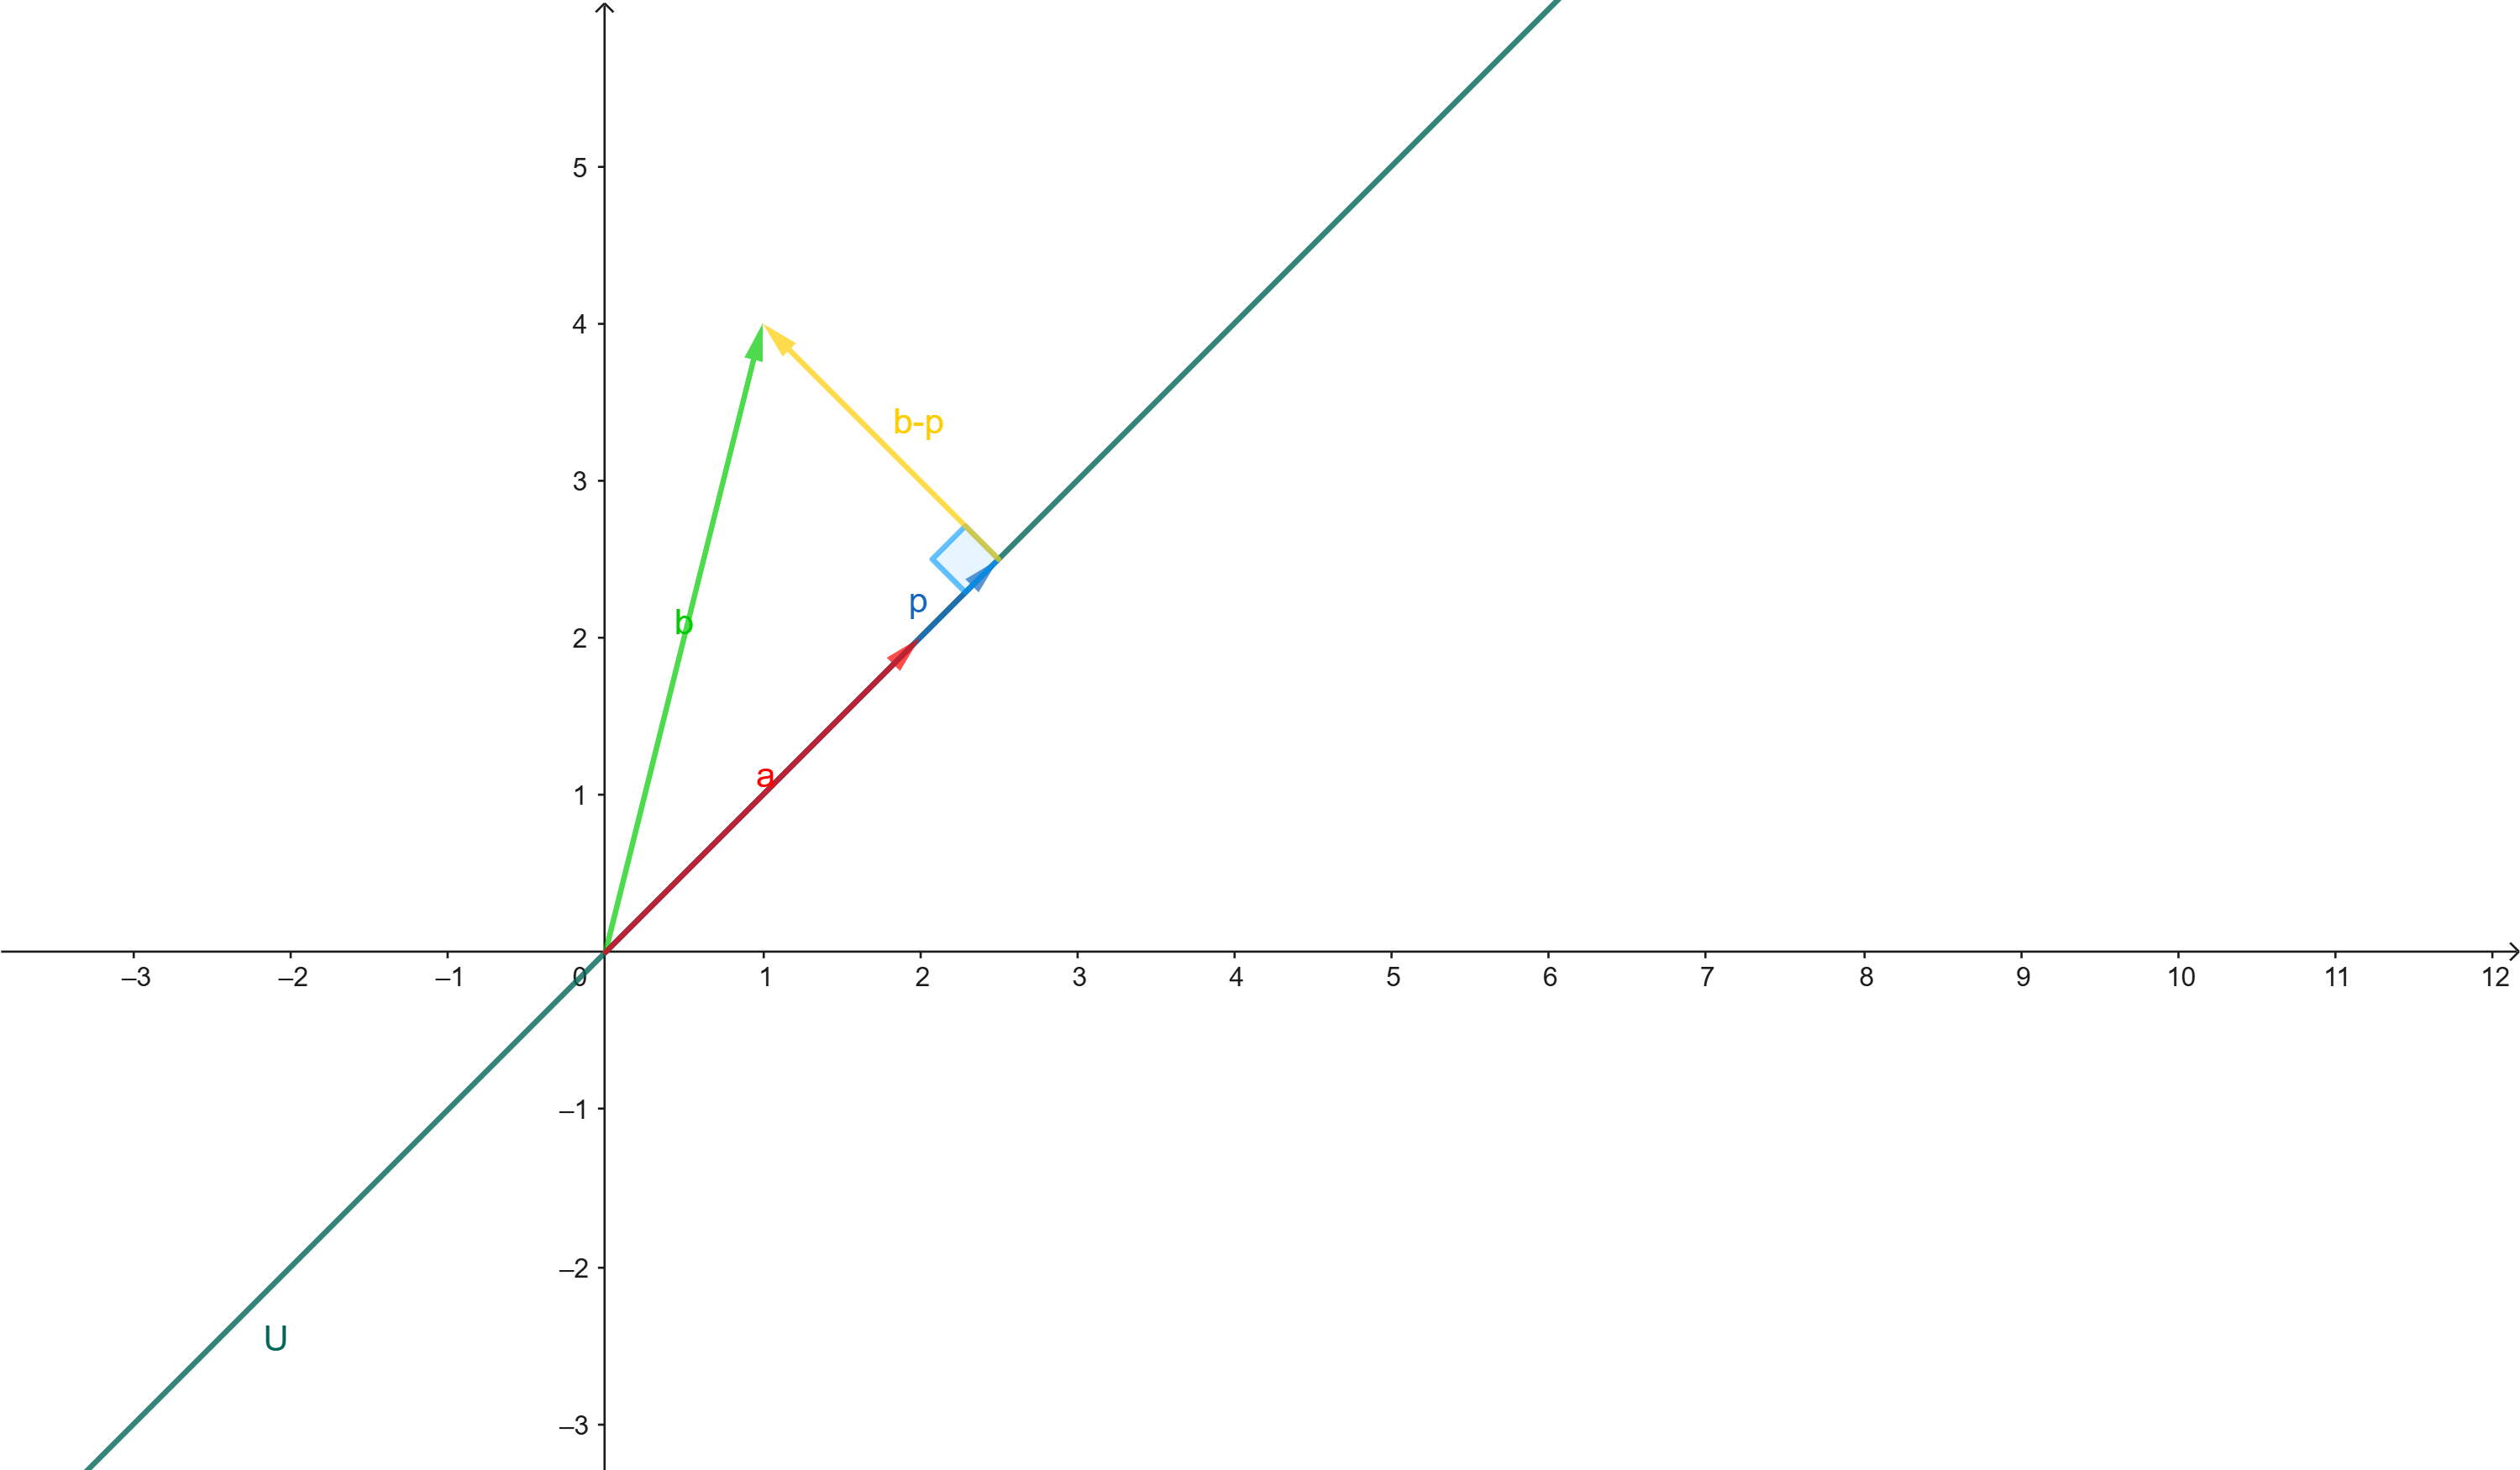
\includegraphics[width=0.7\linewidth]{imgs/alglin-10-projecao-2}
	\caption[Projeção ortogonal em $\mathbb{R}^2$]{Projeção ortogonal em $\mathbb{R}^2$ (arquivo pessoal)}
	\label{fig:alglin-10-projecao-2}
\end{figure}

Vamos então procurar $p$. Nós sabemos que $p = xa$, onde $x$ é um escalar real. Então, nós precisamos determinar $x$ tal que $a^T(b - xa) = 0$. Façamos as contas:

$$
a^T(b - xa) = 0\iff a^Tb - xa^Ta = 0\iff xa^Ta = a^Tb\iff x = \dfrac{a^Tb}{a^Ta}.
$$

Logo, nós temos que $p = \dfrac{a^Tb}{a^Ta}a$. Como $\dfrac{a^Tb}{a^Ta}$ é um escalar, nós podemos escrever $p = a\dfrac{a^Tb}{a^Ta}$ e, pela associatividade, segue que $p = \dfrac{aa^T}{a^Ta}b$. No entanto, $\dfrac{aa^T}{a^Ta}$ é uma matriz de posto $1$. Denotando esta matriz por $P$, segue que este processo pode ser descrito matricialmente por $p = Pb$. A matriz $P$ pertence a uma classe especial de matrizes que nós chamamos de matrizes de projeção, e, neste caso, a uma classe mais especial ainda de matrizes que nós chamamos de matrizes de projeção ortogonal. Então, vamos definir formalmente estas duas classes de matrizes.

\begin{Definition}[Matriz de projeção]
	Uma matriz $P$ é dita uma \textbf{matriz de projeção} quando $P^2 = P$.
\end{Definition}

A intuição de $P^2 = P$ é muito simples. Se nós temos um vetor $x$, e aplicamos uma matriz de projeção $P$ nele, nós obtemos um certo vetor $Px$. Se nós aplicamos a mesma matriz de projeção a este vetor $Px$ (ou seja, fazemos $P^2x$), nós precisamos encontrar o mesmo vetor $Px$, já que um vetor projetado sobre si mesmo pela mesma matriz de projeção é igual ao próprio vetor. De $P^2 = P$, seguirá imediatamente que $P^n = P$ para qualquer $n\in\mathbb{N}$, o que condiz perfeitamente com a nossa intuição.

\begin{Definition}[Matriz de projeção ortogonal]
	Uma matriz $P$ é dita uma \textbf{matriz de projeção ortogonal} quando $P^2 = P$ e $P^T = P$.
\end{Definition}

Vamos, então, mostrar que a matriz de posto $1$ que nós encontramos anteriormente é, de fato, uma matriz de projeção ortogonal (generalizando para $\mathbb{R}^n$).

\begin{Proposition}
	Dados dois vetores $a,b\in\mathbb{R}^n$, a matriz $P = \dfrac{aa^T}{a^Ta}$ é uma matriz de projeção ortogonal.
\end{Proposition}

\begin{Proof}
	Primeiro, vamos mostrar que $P^2 = P$. De fato:
	
	$$
	P^2 = \dfrac{aa^T}{a^Ta}\cdot\dfrac{aa^T}{a^Ta} = \dfrac{a(a^Ta)a^T}{a^Taa^Ta} = \dfrac{(a^Ta)aa^T}{(a^Ta)a^Ta} = \dfrac{aa^T}{a^Ta} = P.
	$$
	Agora, nós vamos mostrar que $P^T = P$. De fato:
	
	$$
	P^T = \left(\dfrac{aa^T}{a^Ta}\right)^T = \dfrac{(aa^T)^T}{a^Ta} = \dfrac{aa^T}{a^Ta} = P.
	$$
	Logo, $P$ é uma matriz de projeção ortogonal.
	
	\qed
\end{Proof}

Agora, nós vamos estender este conceito para um caso mais geral. Nós já sabemos projetar sobre uma reta. Agora, nós queremos aprender a projetar sobre um plano (ou, melhor ainda, sobre um hiperplano).

Suponha que $\{a_1, \cdots, a_k\}$ é uma base para um certo hiperplano, e existe um certo vetor $b$ que não pertence a este hiperplano. Nós queremos encontrar $\{x_1, \cdots, x_k\}$ tais que o vetor $p$ projetado ortogonalmente possa ser escrito como $p = x_1a_1 + \cdots + x_ka_k$. Note que:

$$
x_1a_1 + \cdots + x_ka_k = \begin{bmatrix}
	a_1 & a_2 & \cdots & a_k
\end{bmatrix}x = Ax,
$$
com $x = \begin{bmatrix}
	x_1 \\
	x_2 \\
	\vdots \\
	x_k
\end{bmatrix}$.

Como o conjunto dos $a_i$'s é uma base para o hiperplano, nós podemos entendê-lo como o espaço coluna de $A$. A ideia agora é a mesma: nós queremos encontrar $x$ tal que $a_i^T(b - Ax) = 0$. Escrevendo esta fórmula de maneira matricial, isto equivale a $A^T(b - Ax) = 0$. Assim sendo, nós obtemos:

$$
A^T(b - Ax) = 0\iff A^Tb - A^TAx = 0\iff A^TAx = A^Tb.
$$

As equações $A^TAx = A^Tb$ são chamadas de equações normais. No caso em que $A^TA$ é invertível (e, por enquanto é, já que estamos considerando $A$ como sendo a matriz cujas colunas formam uma base para o hiperplano, mas, generalizando para qualquer $A$, poderia não ser), nós obtemos $x = (A^TA)^{-1}A^Tb$, e, como $p = Ax$, nós obtemos a matriz de projeção ortogonal $P = A(A^TA)^{-1}A^T$.

Nós não provaremos que esta matriz é, de fato, uma matriz de projeção ortogonal, mas, como todo escritor meio preguiçoso gosta de fazer, e eu também, esta demonstração será um dos exercícios para o leitor.

Existe um motivo a mais pelo qual projeções ortogonais são legais: todo vetor de um espaço $E$ pode ser escrito de forma única como a soma de um vetor em um certo subespaço $V$ com um vetor no complemento ortogonal $V^\perp$. Então, seja $x\in E$. Se nós encontramos a projeção ortogonal de $x$ sobre $V$, é muito fácil encontrar a sua projeção sobre $V^\perp$: basta fazer uma subtração.

Mas vamos fazer isto de maneira formal: Considere uma matriz $A_{m\times n}$ tal que $A^TA$ é inversível. Nós sabemos que $C(A)\perp N(A^T)$, ou seja, $\dim C(A) + \dim N(A^T) = m$. Nós queremos projetar um certo vetor $b\in\mathbb{R}^m$ qualquer sobre $C(A)$ e também sobre $N(A^T)$. Suponha que $P$ é a matriz de projeção sobre $C(A)$. Então, pelo Teorema da Decomposição Ortogonal, nós temos que $b$ pode ser escrito de forma única como $b = Pb + p^\perp$, onde $p^\perp\in N(A^T)$. Resolvendo a equação, segue imediatamente que $p^\perp = b - Pb$. Sabemos, porém, que:

$$
b - Pb = Ib - Pb = (I - P)b.
$$
Logo, se $P$ projeta $b$ sobre $C(A)$, então a matriz $I - P$ projeta $b$ sobre $N(A^T)$. De fato, como falamos antes, conhecendo $b$ e $Pb$, encontrar a projeção de $b$ sobre $N(A^T)$ se resume a fazer uma subtração. Mas focar no aspecto matricial dessas operações: queremos provar que $I - P$ é uma matriz de projeção ortogonal.

\begin{Proposition}
	Sejam $A_{m\times n}$ uma matriz tal que $A^TA$ é invertível e $P$ a matriz de projeção ortogonal sobre $C(A)$. Então, $I - P$ é uma matriz de projeção ortogonal sobre $N(A^T)$.
\end{Proposition}

\begin{Proof}
	Primeiro, nós vamos provar que $(I - P)^2 = I - P$. De fato:
	
	$$
	(I - P)^2 = (I - P)(I - P) = I^2 -IP - PI + P^2 = I - 2P + P = I - P.
	$$
	Agora, nós vamos provar que $(I - P)^T = (I - P)$. De fato:
	
	$$
	(I - P)^T = I^T - P^T = I - P.
	$$
	Finalmente, vamos provar que $I - P$ projeta sobre $N(A^T)$. Seja $b\in\mathbb{R}^m$ um vetor qualquer. Então:
	
	\begin{align*}
		A^T((I - P)b) &= A^T(b - Pb) = A^Tb - A^TPb = A^Tb - A^T(A(A^TA)^{-1}A^T)b \\ &= A^Tb - (A^TA)(A^TA)^{-1}A^Tb = A^Tb - A^Tb = 0.
	\end{align*}
	Logo, $I - P$ é uma matriz de projeção ortogonal sobre $N(A^T)$.
	
	\qed
\end{Proof}

Para não ficarmos unicamente presos à teoria, vamos fazer um exemplo:

\begin{Example}
	Considere $A = \begin{bmatrix}
		1 & 2 \\
		3 & 2 \\
		0 & 1
	\end{bmatrix}$ e $b = \begin{bmatrix}
		1 \\
		0 \\
		0
	\end{bmatrix}$. Nós queremos encontrar o vetor $p$ que é a projeção ortogonal de $b$ sobre $C(A)$ e o vetor $p^\perp$ que é a projeção ortogonal de $b$ sobre $N(A^T)$. 
	
	Para encontrar $p$, nós não vamos achar $A(A^TA)^{-1}A^T$, pois não queremos inverter matrizes. Ao invés disso, usaremos as equações normais, resolveremos os sistemas lineares para encontrar $x$ e, por fim, calcularemos $p = Ax$. Recordando, as equações normais são dadas por $A^TAx = A^Tb$. Assim sendo, vamos calcular $A^TA$ e $A^Tb$:
	
	$$
	A^TA = \begin{bmatrix}
		1 & 3 & 0 \\
		2 & 2 & 1
	\end{bmatrix}\begin{bmatrix}
		1 & 2 \\
		3 & 2 \\
		0 & 1
	\end{bmatrix} = \begin{bmatrix}
		10 & 8 \\
		8 & 9
	\end{bmatrix}
	$$
	
	$$
	A^Tb = \begin{bmatrix}
		1 & 3 & 0 \\
		2 & 2 & 1
	\end{bmatrix}\begin{bmatrix}
		1 \\
		0 \\
		0
	\end{bmatrix} = \begin{bmatrix}
		1 \\
		2
	\end{bmatrix}.
	$$
	Assim sendo, nós obtemos o sistema
	
	$$
	\begin{bmatrix}
		10 & 8 \\
		8 & 9
	\end{bmatrix}\begin{bmatrix}
		x_1 \\
		x_2
	\end{bmatrix} = \begin{bmatrix}
		1 \\
		2
	\end{bmatrix}.
	$$
	A solução deste sistema é $x = \begin{bmatrix}
		-7/26 \\
		12/26
	\end{bmatrix}$. Assim sendo, nós encontramos o vetor $p$ fazendo:
	
	$$
	p = Ax = \begin{bmatrix}
		1 & 2 \\
		3 & 2 \\
		0 & 1
	\end{bmatrix}\begin{bmatrix}
		-7/26 \\
		12/26
	\end{bmatrix} = \begin{bmatrix}
		17/26 \\
		3/26 \\
		12/26
	\end{bmatrix} = \dfrac{1}{26}\begin{bmatrix}
		17 \\
		3 \\
		12
	\end{bmatrix}.
	$$
	
	Por sua vez, para achar a projeção ortogonal de $b$ sobre $N(A^T)$, basta fazer 
	
	$$
	p^\perp = b - p = \begin{bmatrix}
		1 \\
		0 \\
		0
	\end{bmatrix} - \begin{bmatrix}
		17/26 \\
		3/26 \\
		12/26
	\end{bmatrix} = \begin{bmatrix}
		9/26 \\
		-3/26 \\
		-12/26
	\end{bmatrix} = \dfrac{1}{26}\begin{bmatrix}
		9 \\
		-3 \\
		-12
	\end{bmatrix}.
	$$
\end{Example}

Em todas as proposições desta seção, nós estávamos considerando que $A^TA$ possui inversa. Agora, no entanto, nós precisamos determinar quando $A^TA$ possui inversa, para que as coisas funcionem como desejamos.

\begin{Theorem}
	Seja $A$ uma matriz $m\times n$. Então, $A^TA$ possui inversa se, e somente se, as colunas de $A$ são LI.
\end{Theorem}

\begin{Proof}
	Nós queremos demonstrar que $N(A^TA) = N(A)$. 
	
	Primeiramente, provaremos que $N(A^TA)\subseteq N(A)$. De fato, $x\in N(A^TA)\iff A^TAx = 0$. Isto implica que
	
	$$
	x^TA^TAx = 0\iff (Ax)^T(Ax) = 0\iff ||Ax||^2 = 0\iff Ax = 0.
	$$
	Logo, $x\in N(A)$.
	
	Agora, provaremos que $N(A)\subseteq N(A^TA)$. De fato:
	
	$$
	x\in N(A)\iff Ax = 0\iff A^TAx = 0.
	$$
	Logo, $x\in N(A^TA)$.
	
	Assim sendo, $N(A^TA) = N(A)$ e, por consequência, $N(A^TA) = \{0\}\iff N(A) = \{0\}$.
	
	\qed
\end{Proof}

\section{Mínimos Quadrados}

Nesta seção, nós vamos desenvolver a primeira grande aplicação de Álgebra Linear. Como nós mencionamos anteriormente, quando o sistema $Ax = b$ não possui solução, nós queremos encontrar um vetor $\tilde{x}$ que esteja o mais próximo possível de ser uma solução do nosso sistema. Vamos adotar uma convenção a partir de agora: toda vez que falarmos em projeção, estaremos falando especificamente em projeção ortogonal.

Vamos desenvolver esta ideia formalmente: considere o sistema $Ax = b$ tal que $b\notin C(A)$ (com $A$ uma matriz $m\times n$ tal que $m > n$). Este sistema linear não possui solução. No entanto, se nós projetarmos $b$ em $C(A)$, o sistema $A\tilde{x} = p$ possuirá solução. Neste caso, o vetor $\tilde{x}$ é ``quase'' uma solução para $Ax = b$. Ele é, na verdade, o vetor que está mais próximo de ser uma solução para $Ax = b$.

Mas como nós medimos o que significa ``estar mais próximo de ser uma solução de $Ax = b$''? É muito simples: quando um sistema linear possui solução, e $x$ é essa solução, nós temos que $||Ax - b|| = 0$. Quando nós encontramos o vetor $\tilde{x}$ que é quase uma solução de um sistema sem solução, nós obtemos $\min_{x\in\mathbb{R}^n}||Ax - b||$. Como, no entanto, trabalhar diretamente com a norma costuma ser difícil, e a norma é sempre maior ou igual a zero, este problema é equivalente a um problema mais fácil:

$$
\min_{x\in\mathbb{R}^n} ||Ax - b||^2.
$$

Este problema é chamado \textbf{Problema de Mínimos Quadrados}. Ele é chamado assim porque nós estamos procurando o vetor $\tilde{x}$ que minimiza o quadrado da norma de $Ax - b$. O vetor $Ax - b$ é chamado de \textbf{resíduo}, e o escalar $||Ax - b||^2$ é chamado de \textbf{erro}.

Vamos agora enunciar e demonstrar a solução do Problema de Mínimos Quadrados.

\begin{Theorem}[Solução do Problema de Mínimos Quadrados]
	Seja $Ax = b$ um sistema linear sem solução, com $A$ sendo uma matriz $m\times n$ tal que $A^TA$ é invertível. Então, a solução do Problema de Mínimos Quadrados é
	
	$$
	\tilde{x} = (A^TA)^{-1}A^Tb.
	$$
\end{Theorem}

\begin{Proof}
	Pelo Teorema da Decomposição Ortogonal, nós podemos escrever $b = p + (b - p)$, onde $p\in C(A)$ é a projeção ortogonal de $b$ em $C(A)$ e $b - p\in N(A^T)$. Assim sendo, nós temos que $Ax - b = (Ax - p) + (b - p)$. Pelo Teorema de Pitágoras, nós temos que:
	
	$$
	||Ax - b||^2 = ||Ax - p||^2 + ||b - p||^2.
	$$
	O nosso objetivo é minimizar $||Ax - b||^2$. Mas note que o termo $||b - p||^2$ não depende de $x$. Assim sendo, este problema equivale a minimizar $||Ax - p||^2$. O vetor $p$ está em $C(A)$, logo, basta achar $x$ tal que $Ax - p = 0$. Fazendo as contas, nós obtemos:
	
	$$
	Ax - p = 0 \implies Ax = p\implies Ax = Pb\implies Ax = A(A^TA)^{-1}A^Tb.
	$$
	Escolhendo $\tilde{x} = (A^TA)^{-1}A^Tb$, nós obtemos $Ax - p = 0$. Logo, a solução de Mínimos Quadrados é $\tilde{x} = (A^TA)^{-1}A^Tb$.
	
	\qed
\end{Proof}

Um exemplo de aplicação direta deste conceito é quando, dado um conjunto de pontos, nós queremos encontrar uma reta que melhor se ajuste a eles (poderia ser uma outra função, mas a regressão linear é melhor para fazer contas na mão). Vamos, assim, fazer um exemplo:

\begin{Example}
	Considere o seguinte conjunto de dados: $\mathcal{D} = \{(0, 1), (1, 1), (2, 3)\}$. Nós queremos encontrar os coeficientes $C$ e $D$ tal que a reta $f(t) = C + Dt$ se ajusta da melhor forma possível aos dados do conjunto $\mathcal{D}$.
	
	Perceba que $f(t) = \begin{bmatrix}
		1 & t
	\end{bmatrix}\begin{bmatrix}
		C \\
		D
	\end{bmatrix}$. Assim sendo, nós podemos considerar a matriz $A$ como:
	
	$$
	A = \begin{bmatrix}
		1 & t_1 \\
		1 & t_2 \\
		1 & t_3
	\end{bmatrix},
	$$
	o vetor $x$ como:
	
	$$
	x = \begin{bmatrix}
		C \\
		D
	\end{bmatrix}
	$$
	e o vetor $b$ como:
	
	$$
	b = \begin{bmatrix}
		y_1 \\
		y_2 \\
		y_3
	\end{bmatrix}.
	$$
	Na prática, isto quer dizer o seguinte: a matriz $A$ é a matriz dos dados de entrada aplicados a cada termo que compõe $f(t)$. O vetor $x$ é o vetor dos coeficientes que nós queremos encontrar, e o vetor $b$ é o vetor dos dados de saída do experimento. Para encontrar o vetor $\tilde{x}$, nós resolvemos as equações normais.
	
	Primeiramente, calculemos $A^TA$:
	
	$$
	A^TA = \begin{bmatrix}
		1 & 1 & 1 \\
		0 & 1 & 2
	\end{bmatrix}\begin{bmatrix}
		1 & 0 \\
		1 & 1 \\
		1 & 2
	\end{bmatrix} = \begin{bmatrix}
		3 & 3 \\
		3 & 5
	\end{bmatrix}.
	$$
	Agora, calculemos $A^Tb$:
	
	$$
	A^Tb = \begin{bmatrix}
		1 & 1 & 1 \\
		0 & 1 & 2
	\end{bmatrix}\begin{bmatrix}
		1 \\
		1 \\
		3
	\end{bmatrix} = \begin{bmatrix}
		5 \\
		7
	\end{bmatrix}.
	$$
	Agora, basta resolver o seguinte sistema linear:
	
	$$
	\begin{bmatrix}
		3 & 3 \\
		3 & 5
	\end{bmatrix}\begin{bmatrix}
		C \\
		D
	\end{bmatrix} = \begin{bmatrix}
		5 \\
		7
	\end{bmatrix}.
	$$
	Fazendo as contas, a solução deste sistema é $\tilde{x} = \begin{bmatrix}
		2/3 \\
		1
	\end{bmatrix}$.
	Logo, a reta que melhor se ajusta ao conjunto $\mathcal{D}$ é $f(t) = \dfrac{2}{3} + t$.
\end{Example}

Vamos mostrar uma imagem representando este exemplo:

\begin{figure}[H]
	\centering
	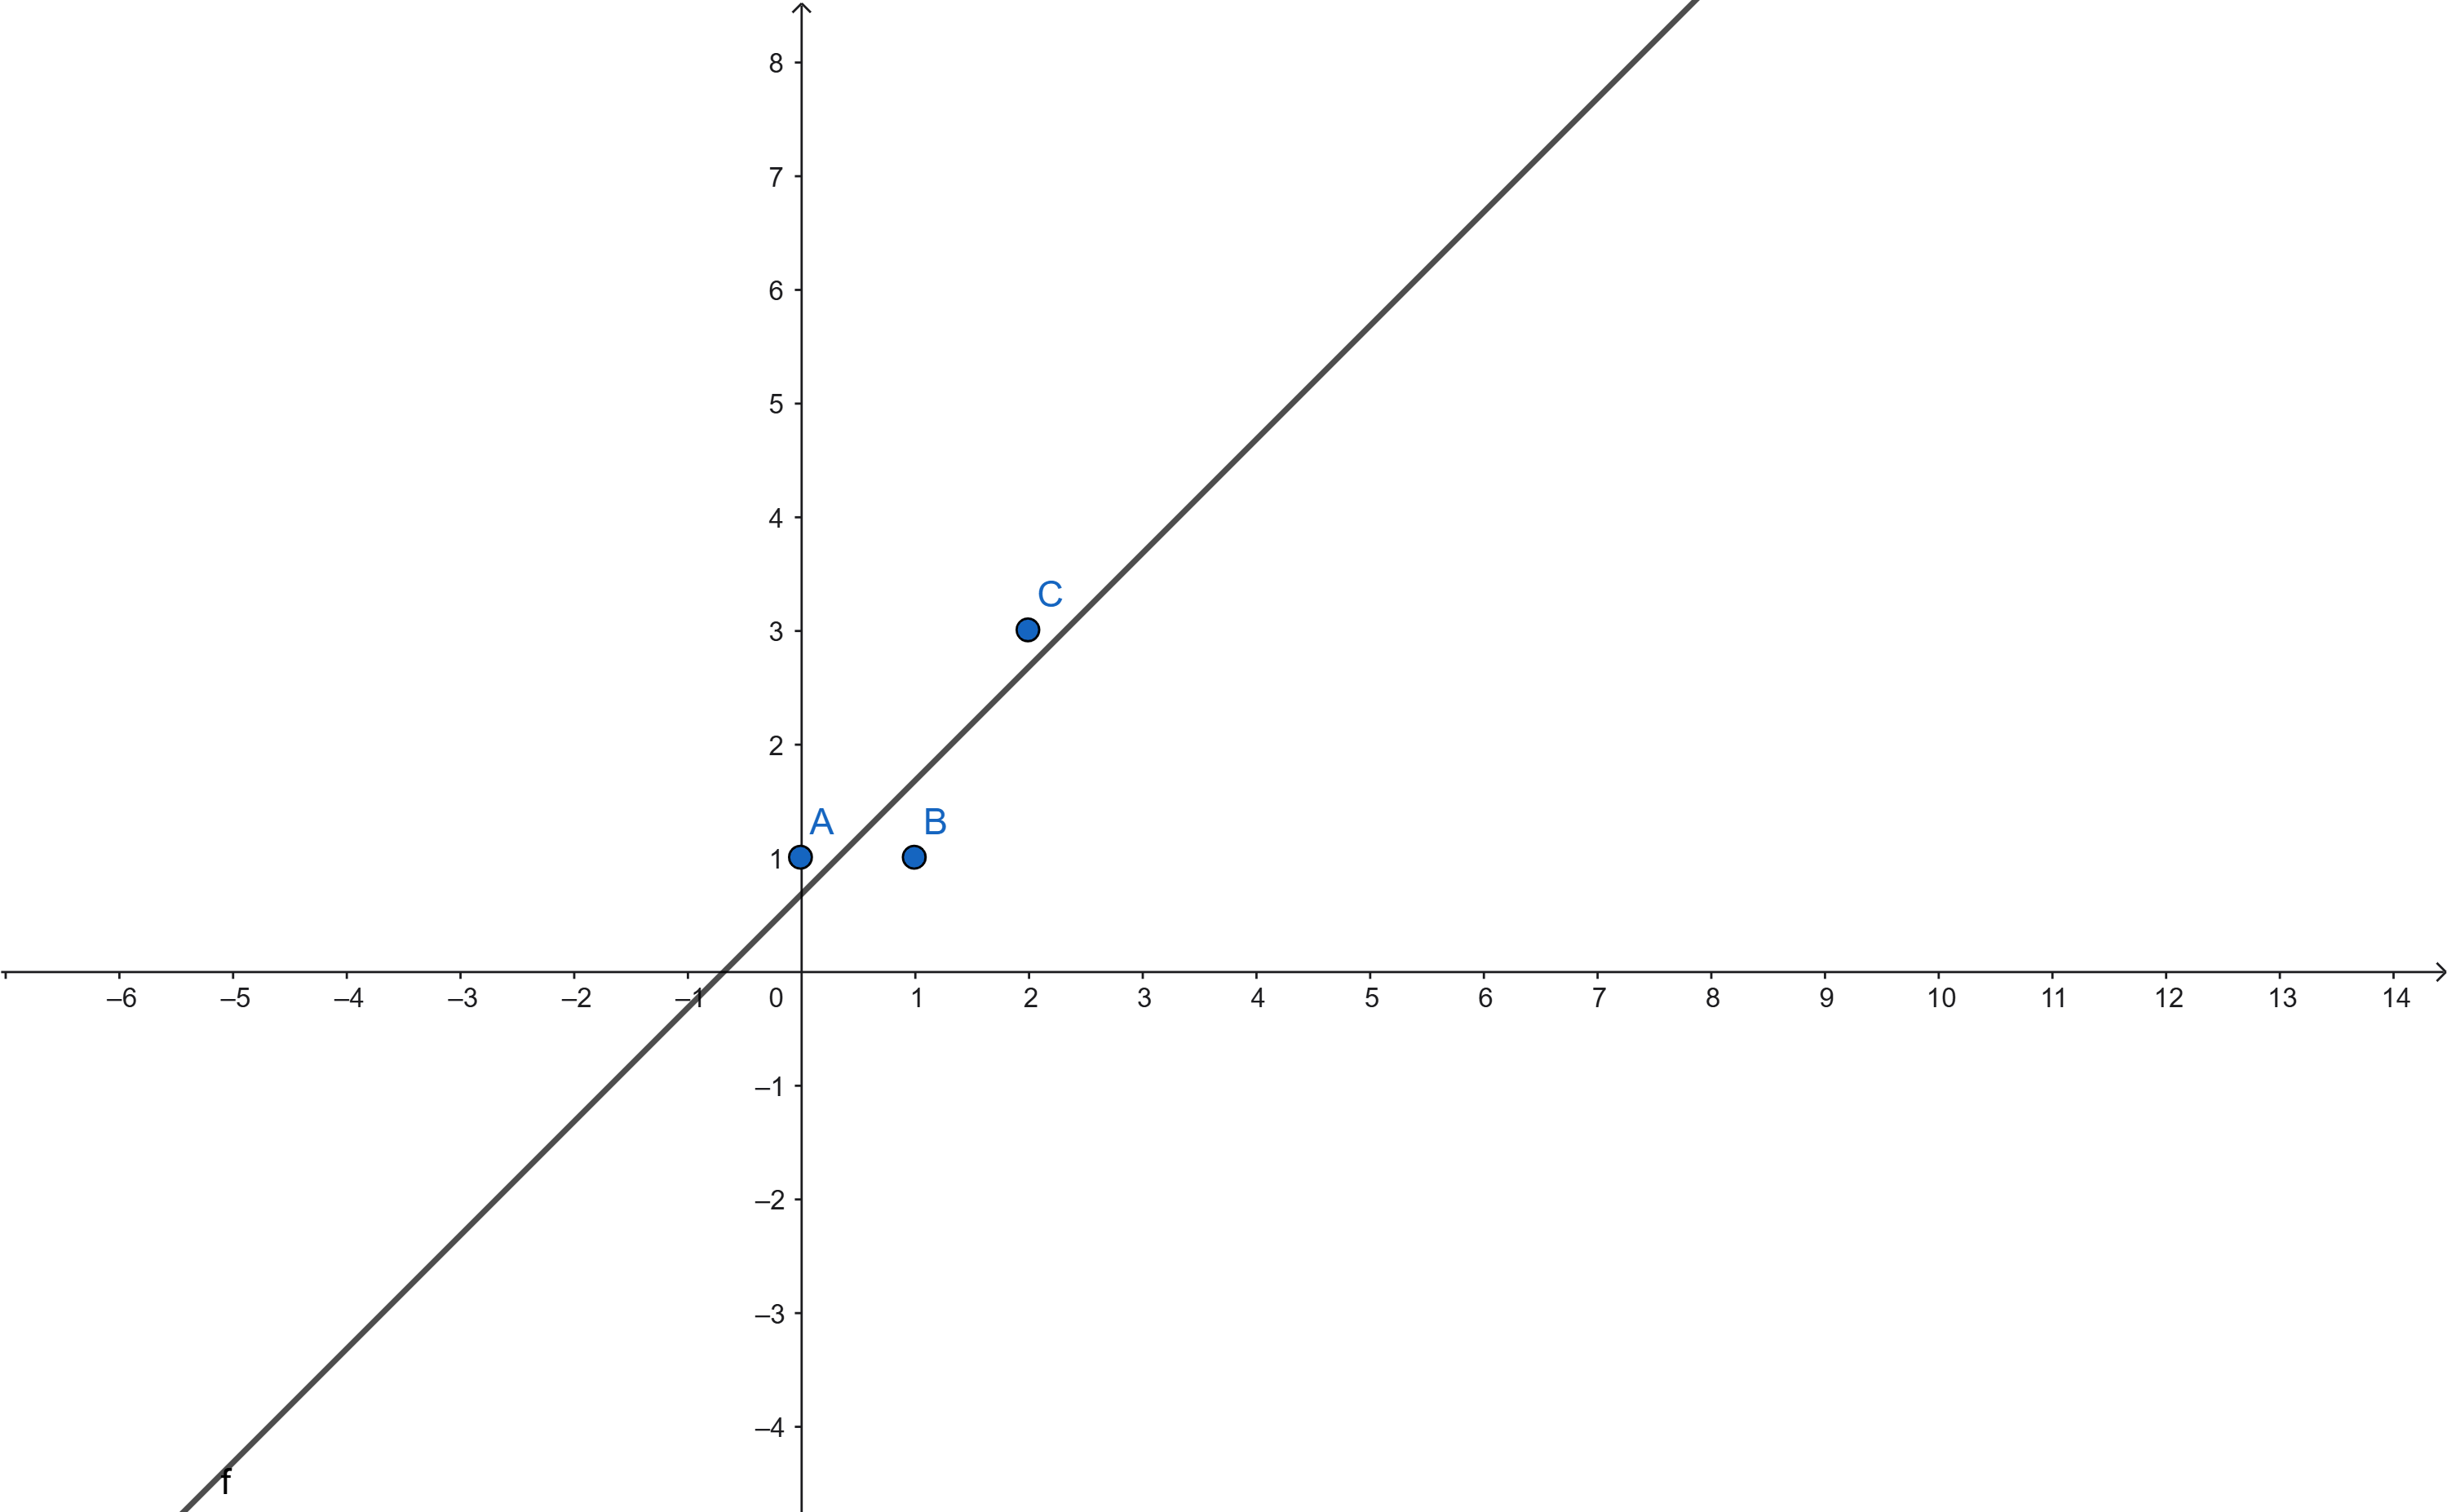
\includegraphics[width=0.7\linewidth]{imgs/alglin-11-regressao-linear}
	\caption[Regressão linear]{Regressão linear (arquivo pessoal)}
	\label{fig:alglin-11-regressao-linear}
\end{figure}


De um modo geral, se nós temos um conjunto de dados $\mathcal{D} = \{(t_1, b_1), (t_2, b_2), \cdots, (t_m, b_m)\}$, e nós queremos ajustá-los por uma reta $f(t) = C + Dt$, nós temos que a matriz $A$ é dada por:

$$
A = \begin{bmatrix}
	1 & t_1 \\
	1 & t_2 \\
	\vdots & \vdots \\
	1 & t_m
\end{bmatrix},
$$
o vetor $x$ é dado por:

$$
x = \begin{bmatrix}
	C \\
	D
\end{bmatrix}
$$
e o vetor $b$ é dado por:

$$
b = \begin{bmatrix}
	b_1 \\
	b_2 \\
	\vdots \\
	b_m
\end{bmatrix}.
$$

A partir daí, basta resolver as equações normais. Explicitamente, nós temos que:

$$
A^TA = \begin{bmatrix}
	1 & 1 & \cdots & 1 \\
	t_1 & t_2 & \cdots & t_m
\end{bmatrix}\begin{bmatrix}
	1 & t_1 \\
	1 & t_2 \\
	\vdots & \vdots \\
	1 & t_m
\end{bmatrix} = \begin{bmatrix}
	m & \sum t_i \\
	\sum t_i & \sum t_i^2
\end{bmatrix}.
$$

e

$$
A^Tb = \begin{bmatrix}
	1 & 1 & \cdots & 1\\
	t_1 & t_2 & \cdots & t_m
\end{bmatrix}\begin{bmatrix}
	b_1 \\
	b_2 \\
	\vdots \\
	b_m
\end{bmatrix} = \begin{bmatrix}
	\sum b_i \\
	\sum t_ib_i
\end{bmatrix}.
$$
Nós podemos transformar $A^TA$ em uma matriz diagonal definindo $s_i = t_i - \overline{t}$, onde $\overline{t} = \frac{1}{m}\sum\limits_{i = 1}^{m} t_i$. Assim sendo, nós obtemos:

$$
A^TA = \begin{bmatrix}
	m & \sum s_i \\
	\sum s_i & \sum s_i^2
\end{bmatrix}.
$$
Nós temos, porém, que:

$$
\sum\limits_{i = 1}^{m} s_i = \sum\limits_{i = 1}^{m}(t_i - \overline{t}) = \sum\limits_{i = 1}^{m} t_i - \sum\limits_{i = 1}^{m}\overline{t} = \sum\limits_{i = 1}^{m} t_i - m\overline{t} = \sum\limits_{i = 1}^{m} t_i - \sum\limits_{i = 1}^{m} t_i = 0.
$$
Assim sendo, segue que:

$$
A^TA = \begin{bmatrix}
	m & 0 \\
	0 & \sum s_i^2
\end{bmatrix}.
$$

Por sua vez, $A^Tb$ transforma-se em:

$$
A^Tb = \begin{bmatrix}
	\sum b_i \\
	\sum s_ib_i
\end{bmatrix}.
$$

Nós obtemos, dessa forma, o sistema linear

$$
\begin{bmatrix}
	m & 0 \\
	0 & \sum s_i^2
\end{bmatrix}\begin{bmatrix}
	C \\
	D
\end{bmatrix} = \begin{bmatrix}
	\sum b_i \\
	\sum s_ib_i
\end{bmatrix}
$$
e, fazendo um pouco de contas, nós obtemos que os coeficientes $C$ e $D$ são dados por:

$$
C = \frac{1}{m}\sum\limits_{i = 1}^{m} b_i = \overline{b}
$$
e

$$
D = \dfrac{\frac{1}{m}\sum\limits_{i = 1}^{m}(t_i - \overline{t})b_i}{\frac{1}{m}\sum\limits_{i = 1}^{m}(t_i - \overline{t})^2}.
$$

\section{Exercícios}
\textbf{Importante:} Alguns dos exercícios são baseados em \cite{lista1doguilherme}, em \cite{axler2026}, em \cite{slide5doyuri}, e em \cite{lista2doguilherme}.

\noindent $\mathbf{7.1)}$ Sejam $x = (x_1, \cdots, x_n)^T$ e $y = (y_1, \cdots, y_n)^T$. Mostre que a função $\langle\cdot,\cdot\rangle:\mathbb{R}^n\times\mathbb{R}^n\to\mathbb{R}$, definida como:

$$
\langle x, y\rangle = x\cdot y = x^Ty = \sum\limits_{i = 1}^{n} x_iy_i
$$
é um produto interno.

$\\$
$\mathbf{7.2)}$ Sejam $p$ e $q$ dois polinômios em $\mathcal{P}_n$. Mostre que a função $\langle\cdot,\cdot\rangle:\mathcal{P}_n\times\mathcal{P}_n\to\mathbb{R}$, definida como:

$$
\langle p, q\rangle = \displaystyle\int_{-1}^{1} p(x)q(x) \,dx
$$
é um produto interno.

$\\$
$\mathbf{7.3)}$ Seja $x = (x_1, \cdots, x_n)^T$. Mostre que a função $||\cdot||:\mathbb{R}^n\to\mathbb{R}$, definida como:

$$
||x|| = \left(\sum\limits_{i = 1}^{n} x_i^2\right)^\frac{1}{2}
$$
é uma norma.

$\\$
$\mathbf{7.4)}$ Seja $x = (x_1, \cdots, x_n)^T$. Mostre que a função $||\cdot||_p:\mathbb{R}^n\to\mathbb{R}$, definida como:

$$
||x||_p = \left(\sum\limits_{i = 1}^{n} x_i^p\right)^\frac{1}{p}
$$
é uma norma, para $1\leq p <\infty$. Quando $0\leq p < 1$, esta função ainda é uma norma? Se sim, justifique; se não, quais axiomas não são satisfeitos?

$\\$
$\mathbf{7.5}$ Seja $x = (x_1, \cdots, x_n)^T$.

a) Mostre que a função $||\cdot||:\mathbb{R}^n\to\mathbb{R}$, definida como:

$$
||x||_{\infty} = \max_{i} |x_i|
$$
é uma norma.

b) Prove que $\lim\limits_{p\to\infty} ||x||_p = ||x||_{\infty}$.

$\\$
$\mathbf{7.6)}$ Seja $V$ um espaço vetorial real munido de um produto interno $\langle\cdot, \cdot\rangle$, e seja $||x|| = \sqrt{\langle x, x\rangle}$ para todo $x\in V$. Mostre que, dados $u,v\in V$ quaisquer, vale a identidade: 

$$
||u + v||^2 + ||u - v||^2 = 2||u||^2 + 2||v||^2.
$$

\textbf{Nota:} Esta identidade é conhecida como Regra do Paralelogramo, e é um resultado mais importante do que parece (e mais forte do que o que o exercício pede para provar): basicamente, é verdade que, se um espaço possui um produto interno, a norma induzida por ele satisfaz essa identidade e, reciprocamente, se um espaço normado satisfaz a Regra do Paralelogramo, então a norma vem de um produto interno. Neste exercício, vocês provarão somente a ida, e os mais curiosos podem tentar demonstrar a volta também, que é conhecida como Teorema de Jordan-von Neumann.

$\\$
$\mathbf{7.7)}$ Sejam $U$ e $V$ dois subespaços vetoriais de $E$. Prove que:

$$
\dim(U + V) = \dim U + \dim V - \dim(U - V).
$$

$\\$
$\mathbf{7.8)}$ Considere o subespaço vetorial $U = \{(x, y, 2x, 3y)^T; x, y\in\mathbb{R}\}\subseteq\mathbb{R}^4$.

a) Verifique que o vetor $x = (1, 2, 2, 6)^T\in U$.

b) Encontre um vetor $y\in\mathbb{R}^4$ tal que $x^Ty = 0$.

c) Determine um subespaço $V$ tal que $U\perp V$ e $y\in V$.

d) Determine as dimensões de $U$ e $V$.

e) Conclua que $\dim U + \dim V \leq \dim\mathbb{R}^4$.

f) Generalize o item e) para qualquer espaço vetorial: prove que, se $E$ é um espaço vetorial, e $U$ e $V$ são dois subespaços de $E$ tais que $U\perp V$, então $\dim U + \dim V \leq \dim E$.

$\\$
$\mathbf{7.9)}$ Seja $V$ um subespaço vetorial de $E$. Prove que o complemento ortogonal de $V$ é único.

$\\$
$\mathbf{7.10)}$ Considere $E = \mathbb{R}^3$. Ache $S^\perp$ para os seguintes conjuntos:

a) $S = \{0\}$.

b) $S = \operatorname{span}\left\{\begin{bmatrix}
	1 \\
	1 \\
	1
\end{bmatrix}\right\}$.

c) $S = \operatorname{span}\left\{\begin{bmatrix}
	1 \\
	1 \\
	1
\end{bmatrix}, \begin{bmatrix}
	1 \\
	1 \\
	-1
\end{bmatrix}\right\}$.

d) $S = \left\{\begin{bmatrix}
	1 \\
	5 \\
	1
\end{bmatrix}, \begin{bmatrix}
	2 \\
	2 \\
	2
\end{bmatrix}\right\}$. Note que $S$ não é um subespaço, mas $S^\perp$ é.

$\\$
$\mathbf{7.11)}$ Suponha que $U$ é um subespaço de $E$. O que é $U + U$?

$\\$
$\mathbf{7.12)}$ Seja $V = \operatorname{span}\left\{\begin{bmatrix}
	2 \\
	0 \\
	1 \\
	3
\end{bmatrix}, \begin{bmatrix}
	5 \\
	-1 \\
	0 \\
	9
\end{bmatrix}\right\}$ um subespaço de $\mathbb{R}^4$, e considere o vetor $x = \begin{bmatrix}
	0 \\
	1 \\
	2 \\
	4
\end{bmatrix}$. Encontre a decomposição ortogonal de $x$.

$\\$
$\mathbf{7.13)}$ Seja $V$ o plano $3x + 2y - z = 0$ em $\mathbb{R}^3$. Considere o vetor $v = \begin{bmatrix}
	5 \\
	4 \\
	-1
\end{bmatrix}$. Ache a decomposição ortogonal de $v$.

$\\$
$\mathbf{7.14)}$ Demonstre que nenhum par de planos $V$ e $W$ em $\mathbb{R}^3$ pode ser ortogonal.

$\\$
$\mathbf{7.15)}$ Seja $A_{m\times n}$ uma matriz tal que $A^TA$ é invertível. Prove que $P = A(A^TA)^{-1}A^T$ é uma matriz de projeção ortogonal.

$\\$
$\mathbf{7.16)}$ Seja $A$ uma matriz $4\times 3$ formada pelas primeiras $3$ colunas da matriz identidade $4\times 4$. Projete o vetor $b = (1, 2, 3, 4)^T$ no espaço coluna de $A$. Ache a matriz de projeção $P$.

$\\$
$\mathbf{7.17)}$ Seja $P$ uma matriz de projeção qualquer.

a) Prove que $C(I - P) = N(P)$.

b) Prove que $N(I - P) = C(P)$.

c) Suponha agora que $P$ é uma matriz de projeção ortogonal. Prove que $N(P) = C(P)^\perp$.

$\\$
$\mathbf{7.18)}$ Projete $b$ sobre o espaço coluna de $A$ resolvendo $A^TA\hat{x} = A^Tb$ e $p = A\hat{x}$ para:

a) $\begin{bmatrix}
	1 & 0 \\
	0 & 1 \\
	1 & 1
\end{bmatrix}$ e $\begin{bmatrix}
	2 \\
	5 \\
	-1
\end{bmatrix}$.

b) $\begin{bmatrix}
	1 & 1 \\
	1 & 0 \\
	1 & 1
\end{bmatrix}$ e $\begin{bmatrix}
	2 \\
	-1 \\
	6
\end{bmatrix}$.

c) $\begin{bmatrix}
	1 & 0 \\
	1 & 0 \\
	1 & 1
\end{bmatrix}$ e $\begin{bmatrix}
	7 \\
	-3 \\
	4
\end{bmatrix}$.

$\\$
$\mathbf{7.19)}$ Considere o conjunto de dados $\mathcal{D} = \{(1, 2), (2, 3), (5, -1)\}$. Encontre a solução de mínimos quadrados $\hat{x} = (C, D)^T$ tal que $y(t) = C + Dt$ é a reta que melhor se ajusta aos dados. Encontre também a projeção $p = A\hat{x}$. Quais dos quatro subespaços fundamentais contêm o vetor erro $e = b - p$? E o vetor $p$? E o vetor $\hat{x}$? Qual é o núcleo de $A$?

$\\$
$\mathbf{7.20)}$ (Desafio!) Reformule o problema de mínimos quadrados para ajustar a função $a + d\cos(t + \theta)$, onde $a, d, \theta$ são os coeficientes a serem calculados.


